\documentclass[UTF8]{article}
\usepackage{geometry}                % See geometry.pdf to learn the layout options. There are lots.
\geometry{a4paper}                   % ... or a4paper or a5paper or ... 

%\geometry{landscape}                % Activate for for rotated page geometry
\usepackage{graphicx}
\usepackage{graphbox}
\usepackage{hyperref}
\usepackage{amssymb}
\usepackage{epstopdf}
\usepackage{algorithm}
\usepackage[noend]{algpseudocode}
\usepackage{enumitem}
\usepackage[acronym]{glossaries}
\usepackage[hang,footnotesize,bf]{caption}
\DeclareGraphicsRule{.tif}{png}{.png}{`convert #1 `dirname #1`/`basename #1 .tif`.png}


% Copied from Stack Exchange for ToDo items
% -----------------------------------------------------------
\usepackage{xargs} 
\usepackage[pdftex,dvipsnames]{xcolor}  % Coloured text etc.
% 
\usepackage[colorinlistoftodos,prependcaption,textsize=tiny]{todonotes}
\newcommandx{\unsure}[2][1=]{\todo[linecolor=red,backgroundcolor=red!25,bordercolor=red,#1]{#2}}
\newcommandx{\change}[2][1=]{\todo[linecolor=blue,backgroundcolor=blue!25,bordercolor=blue,#1]{#2}}
\newcommandx{\info}[2][1=]{\todo[linecolor=OliveGreen,backgroundcolor=OliveGreen!25,bordercolor=OliveGreen,#1]{#2}}
\newcommandx{\improvement}[2][1=]{\todo[linecolor=Plum,backgroundcolor=Plum!25,bordercolor=Plum,#1]{#2}}
\newcommandx{\thiswillnotshow}[2][1=]{\todo[disable,#1]{#2}}


\title{Validator Economics: Variable min validator deposit size\\
\vspace{4pt}
\large EF Academic Grant ID: FY23-1030\\
\vspace{16pt}
DATA SOURCES \& GATHERING}
\vspace{16pt}
\author{Sandra Johnson\\
ConsenSys Software R\&D}
\date{\today}                                           % Activate to display a given date or no date

\begin{document}
\maketitle


% Acronym definitions
\newacronym{apr}{APR}{annual percentage rate}
\newacronym{ef}{EF}{Ethereum Foundation}
\newacronym{mev}{MEV}{maximal extractable value}
\newacronym{rig}{RIG}{Rigorous Incentives Group}
\newacronym{ssf}{SSF}{single slot finality}

% ------------------------------------------------------------------------------
\section{Overview}
% ------------------------------------------------------------------------------
This document is joint work with Kerrie Mengersen and Patrick O'Callaghan, and details available information, data sources, and proposed visualisations that will provide relevant data insights to gain a deeper understanding of current validator economics and any intuitions or assumptions used in formulating proposed solutions to capping the number of validators. 

The information gathering is targeted towards the proposal being evaluated, viz. a variable minimum validator balance, which is one of the proposals that Vitalik articulated in his blog post regarding \gls{ssf} 

As the project progresses and additional data requirements are identified, this document will be updated accordingly.

Many people have generously contributed time and data, and made helpful suggestions, which has been incredibly helpful in compiling the resources listed in this document. They include, but are not limited to Barnabé Monnot and the \gls{rig} team, Justin Drake, Alexander Tesfamichael, Ben Edgington, Paul Harris and Josh Fernandez.

\section{Data Sources}
% ==================
\label{sec:sources}
% ---------------------------------------------------------------
\subsection{Key data points}
% --------------------------------------------------------------
\begin{itemize}
\item The beacon chain \textbf{deposit contract address} is: 0x00000000219ab540356cBB839Cbe05303d7705Fa 
\item The beacon chain \textbf{genesis block number} is 11182202
\end{itemize}

% ----------------------------------------------------------
\subsection{Client and staking pool diversity}
% ---------------------------------------------------------
\label{sec:diversity}
\begin{itemize}
	\item \textit{\href{https://clientdiversity.org/}{Diversify Now}} dashboard by \textit{\href{https://etheralpha.org/}{Ether alpha}} displays the current client distribution in the Consensus and Execution layers. (Figure~\ref{fig:CLELdiversity}, page~\pageref{fig:CLELdiversity}).
	\item \textit{\href{https://migalabs.es/beaconnodes}{Beacon Chain Network Public Dashboard}} by \textit{\href{https://migalabs.es/}{Miga Labs}} has several visualisations: 
	\begin{itemize}
		\item Client diversity  (Figure~\ref{fig:diversity}(a), page~\pageref{fig:diversity})
		\item Client diversity evolution (Beacon chain client distribution over time) (Figure~\ref{fig:diversity}(b), page~\pageref{fig:diversity})
		\item OS distribution of active nodes (Figure~\ref{fig:active}(a), page~\pageref{fig:active})
		\item Geographical representation of client evolution over time  (Figure~\ref{fig:active}(b), page~\pageref{fig:active})
		\item Active nodes round trip time distribution (RTT) (Figure~\ref{fig:rtt}(a), page~\pageref{fig:rtt})
		\item Graphical distribution (Beacon chain node distribution)  (Figure~\ref{fig:rtt}(b), page~\pageref{fig:rtt})
		\item RTT distribution (Figure~\ref{fig:aass}(a), page~\pageref{fig:aass})
		\item Advertised attestation subnets subscription (Figure~\ref{fig:aass}(b), page~\pageref{fig:aass})
		\item Number of beach nodes per IP (Figure~\ref{fig:ipdist}), page~\pageref{fig:ipdist})
	\end{itemize}
However, it is important to note that it is challenging to measure peer types in the network, and therefore the figures are at best approximations based on the information at hand. 

\end{itemize}	
% ---------------------------------------------------------
 \subsection{Total ETH Supply}
 % ---------------------------------------------------------
\label{sec:ethsupply} 
        The total supply of ETH used to be fairly simple to work out, but it is now more complicated for two main reasons:  implementation of EIP-1559 and the Merge.
Currently we are ``(a) burning ETH via the base fee and (b) the issuance is variable depending on the number of validators.'' (Ben Edgington 2023). 
\begin{itemize}
	\item Ultrasound is considered a credible source for total ETH supply projections. \\\textit{\href{https://ultrasound.money/}{Ultra sound money}} visualises various aspects of Ether supply since the Merge, gas, supply projections, the burn, total value secured - TVS and monetary premium. \\
Ultrasound supplied two datasets - the first had total supply at a more accurate and finer grained level, but shorter time period and the second dataset had data points roughly every 1,000 epochs covering from soon after Beacon chain genesis. The latter dataset is from Glassnode and would not be as accurate as the initial data provided by Alex Tesfamichael from Ultrasound.
	\item \textit{\href{https://etherscan.io/chart/ethersupplygrowth}{Etherscan}} is a good source of historic data for the growth in Ether supply since 2015.
\end{itemize}
% ---------------------------------------------------------	
\subsection{Multiple datasets}
% ---------------------------------------------------------
There are several resources that contain lists and visualisations of a variety of data from Ethereum Mainnet. Obtaining the raw data used on the websites and dashboards are not always easily accessible.
\label{sec:multiple}
\begin{itemize}
	\item \textit{\href{https://beaconcha.in/}{beaconcha.in}}, an open source Ethereum explorer, is a rich and informative resource providing visualisations and summary statistics of various aspects of the chain. It is not clear if it is possible to gain access to the data used to generate the many graphs and summary statistics. The website currently contains the following:
	\begin{itemize}
		\item On the home page, there is a \textbf{progress line} at the top of the page showing the \textit{number of slots left in the current epoch}.
		\item Immediately below the progress line, there is a \textbf{summary line} showing the \textit{current epoch number}, the \textit{last finalised epoch}, the \textit{current slot number}, the \textit{number of active and pending validators}, the \textit{total staked ETH} and the \textit{average validator balance}. 
		\item Below this summary there is a \textbf{graph} of the \textit{number of active validators} and \textit{staked ETH} for the last week (Figure xx on page xx).
		\item Then there are two side by side tables. The \textbf{left table} has information about the most recent epochs: \textit{epoch number, time, whether it is final, the eligible ETH, the number of percentage of votes}. The \textbf{right table} has information about the most recent blocks: \textit{epoch number, slot number, block number, status of the block (proposed or missed), time} and the \textit{proposer id}. These two tables are shown in Figure xx on page xx.\\
		\item Moreover, one can click on the epoch, slot and block numbers in the tables to obtain a detailed view of the epoch, slot or block number (Figures xxx - yyy). 
		\item There is also a link to the validator ID in the right table that provides a detailed view of that validator (Fig zz).
		\item 
	\end{itemize}

	\item \textit{\href{https://mevboost.pics/data.html}{Mevboost.pics - Open Data}} will eventually provide links to download several datasets: 
		\begin{itemize}
			\item \textit{eth\_data} - Slots since Merge with additional MEV-Boost and validator info such as: date, slot, block number, relay, builder pubkey, proposer pubkey, mevboost value, builder, validator \textit{(Available now)}
			\item \textit{pubkey\_mapping} - Validator public keys mapped to known entities such as Lido, Kraken ect. \textit{(Not available)}
			\item \textit{tc\_txs} - Tornado Cash related transactions \textit{(Not available)}
			\item \textit{staking\_txs} - Deposit transactions to the ETH2 Deposit contract \textit{(Not available)}
			\item \textit{relays\_over\_time} - Number of successfully relayed blocks per day \textit{(Not available)}
			\item \textit{builders\_over\_time} - Number of successfully built blocks per day \textit{(Not available)}
		\end{itemize}
\end{itemize}
% ---------------------------------------------------------
\subsection{Stakers and Staking pools}
% ---------------------------------------------------------
\label{sec:stakers}
\begin{itemize}
	\item \textbf{Data from an archive node} \\
	We had access to a teku-besu archive node, \texttt{teku-besu-ohio-mainnet-archive-01},  against which we were able to run many API queries to provide some rich data.\\
	 We ran API calls from those listed in GitHub: \href{https://ethereum.github.io/beacon-APIs/?urls.primaryName=dev}{Eth Beacon Node API}
\end{itemize}

% ---------------------------------------------------------------
\subsection{Existing visualisations}
% --------------------------------------------------------------
\subsubsection*{Client diversity}
% --------------------------------------

\begin{figure}[htbp]
\begin{center}
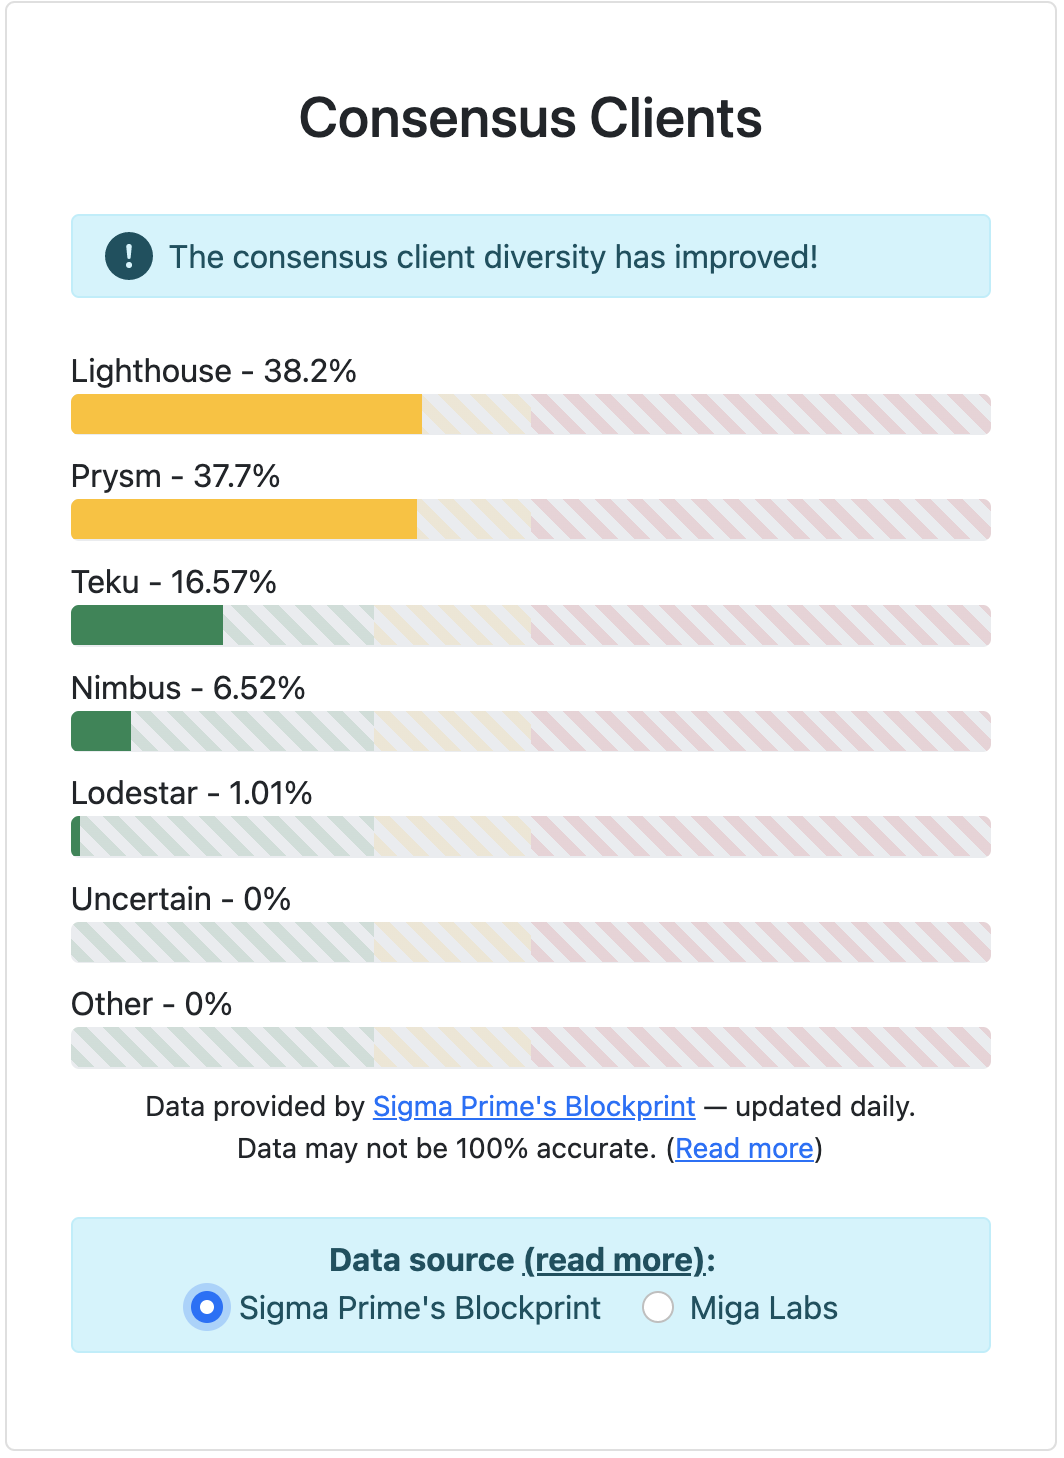
\includegraphics[width=0.3\linewidth, align=c]{images/CL-sigma}
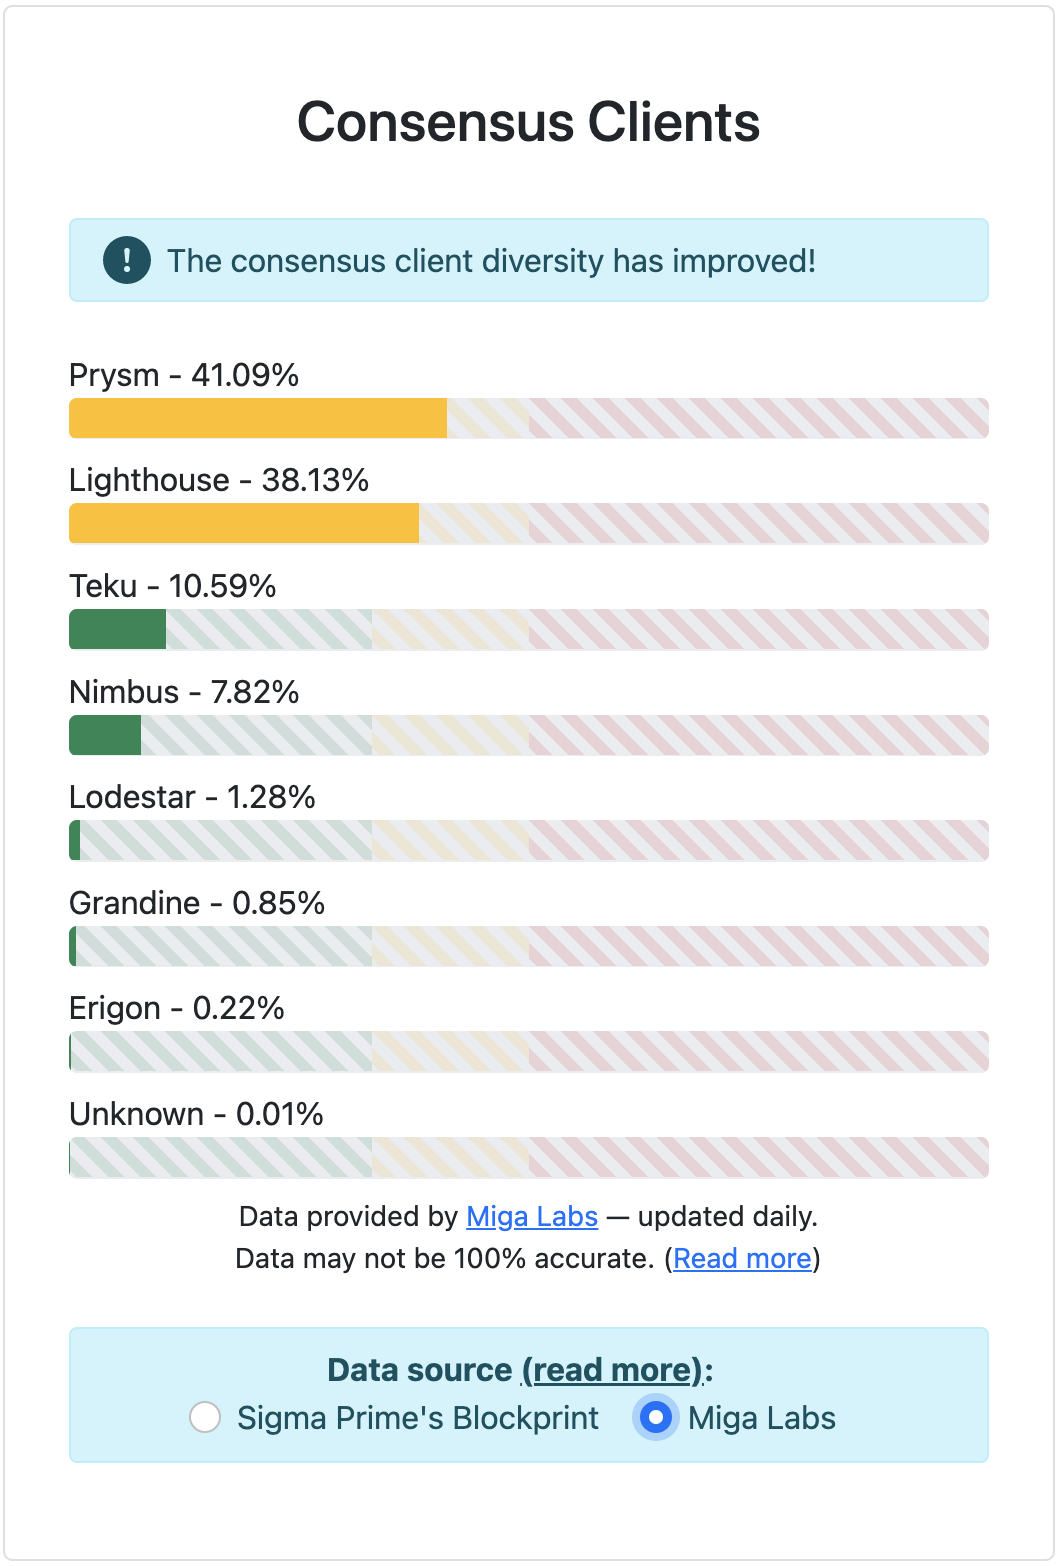
\includegraphics[width=0.3\linewidth, align=c]{images/CL-migalabs}
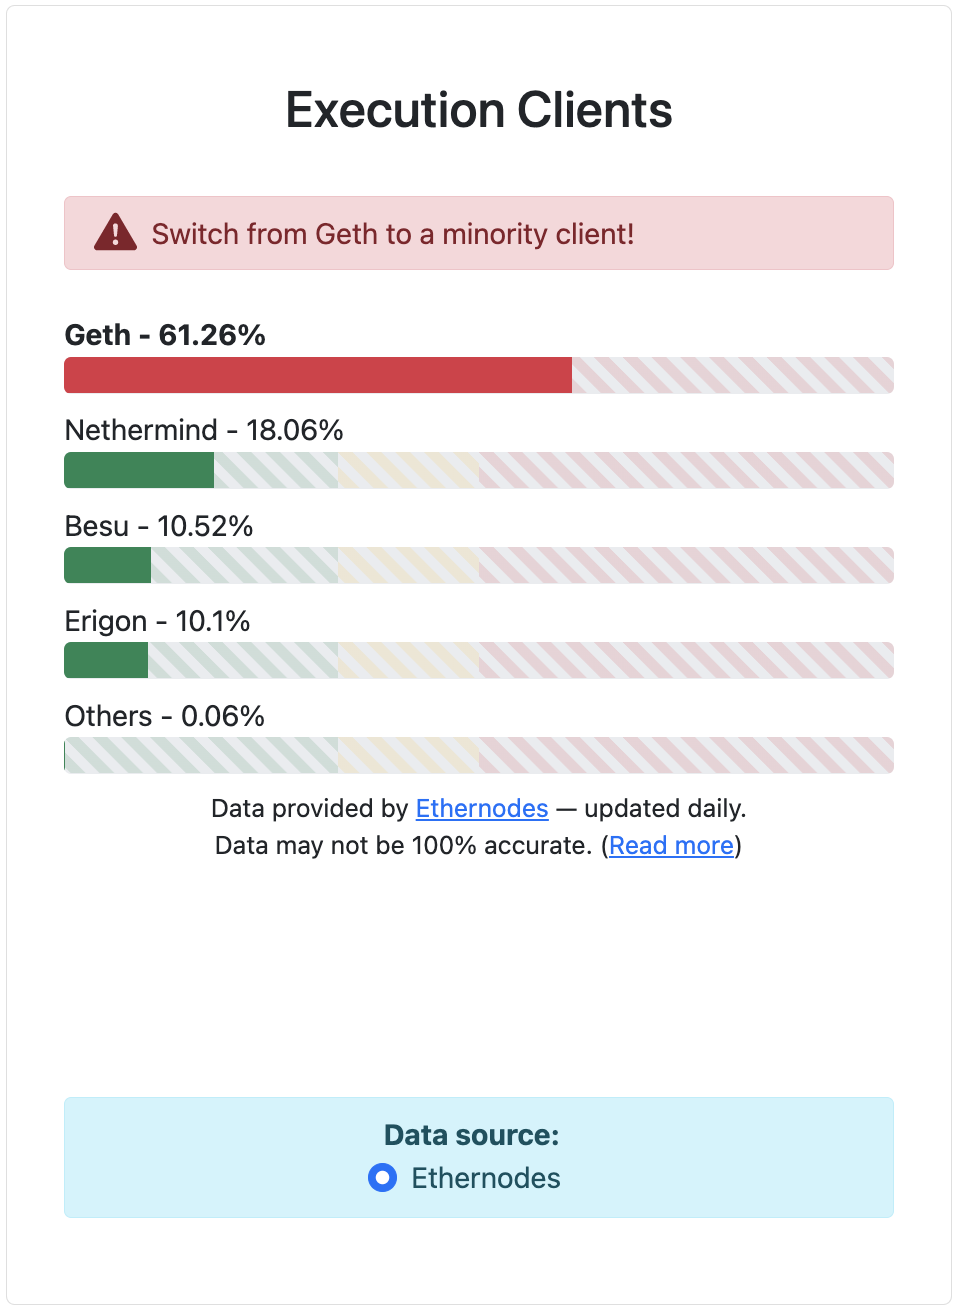
\includegraphics[width=0.3\linewidth, align=c]{images/EL-diversity}\\
(a)\hspace{110pt}        (b)\hspace{110pt} (c)\\
\caption{Consensus layer client diversity using Sigma Prime's Blockprint data (a) and using Migalabs data (b). Execution layer client diversity using Ethernodes data (19 May 2023)}
\label{fig:CLELdiversity}
\end{center}
\end{figure}

 \begin{figure}[htbp]
\begin{center}
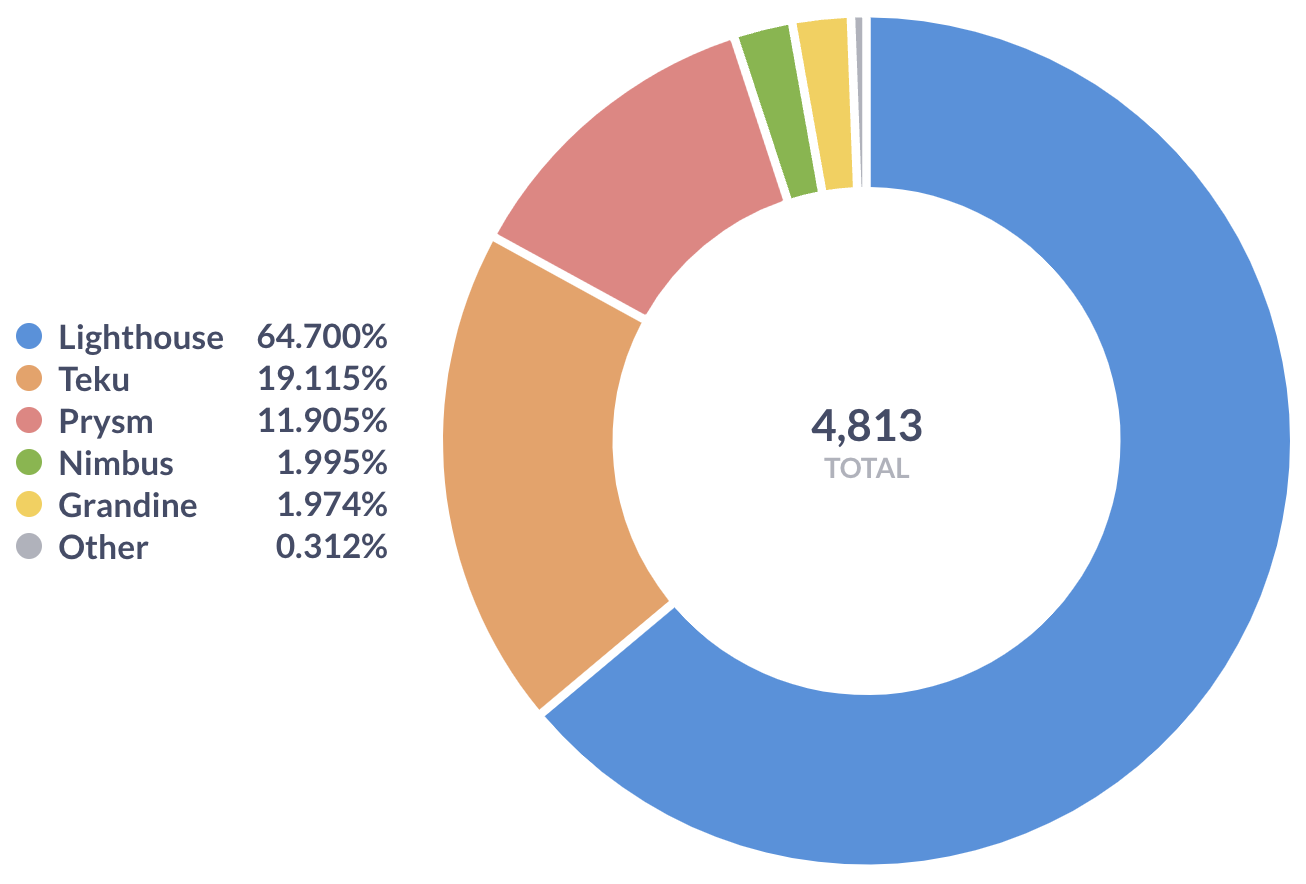
\includegraphics[width=0.48\linewidth]{images/clientdiversity}
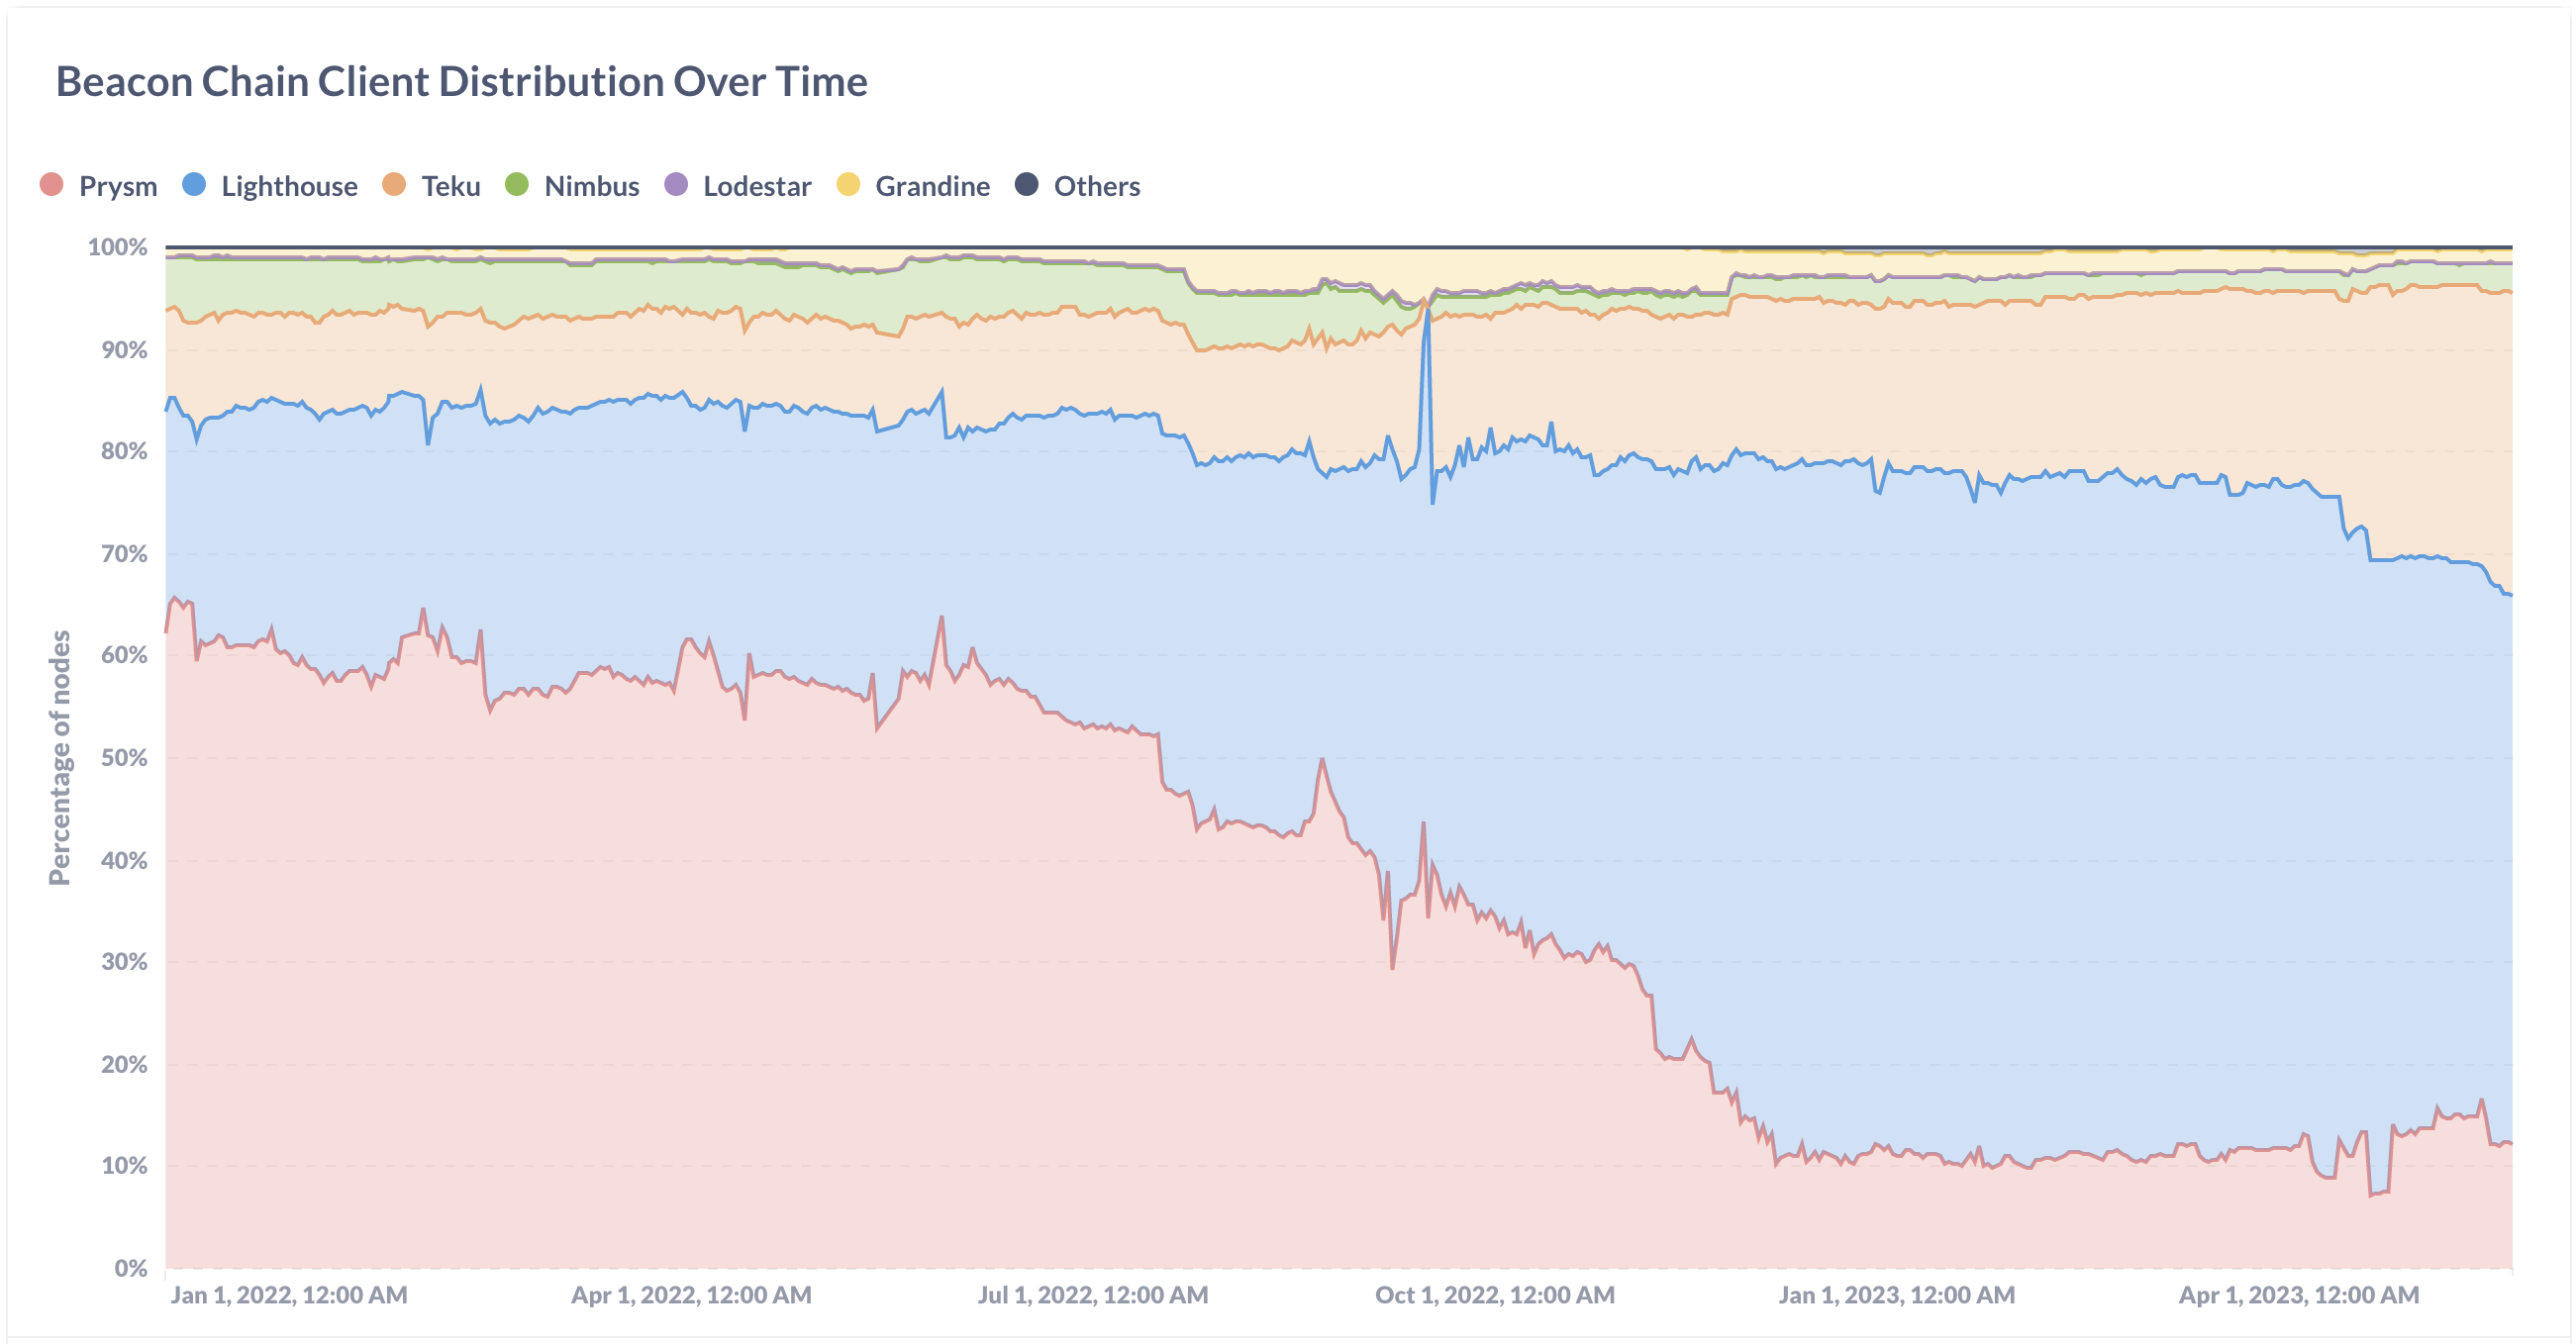
\includegraphics[width=0.48\linewidth]{images/architecture} \\
(a)\hspace{160pt}        (b)\\
\caption{Beacon chain client diversity from Migalabs (a) and client distribution over time (b) (9 May 2023)}
\label{fig:diversity}
\end{center}
\end{figure}

\begin{figure}[htbp]
\begin{center}
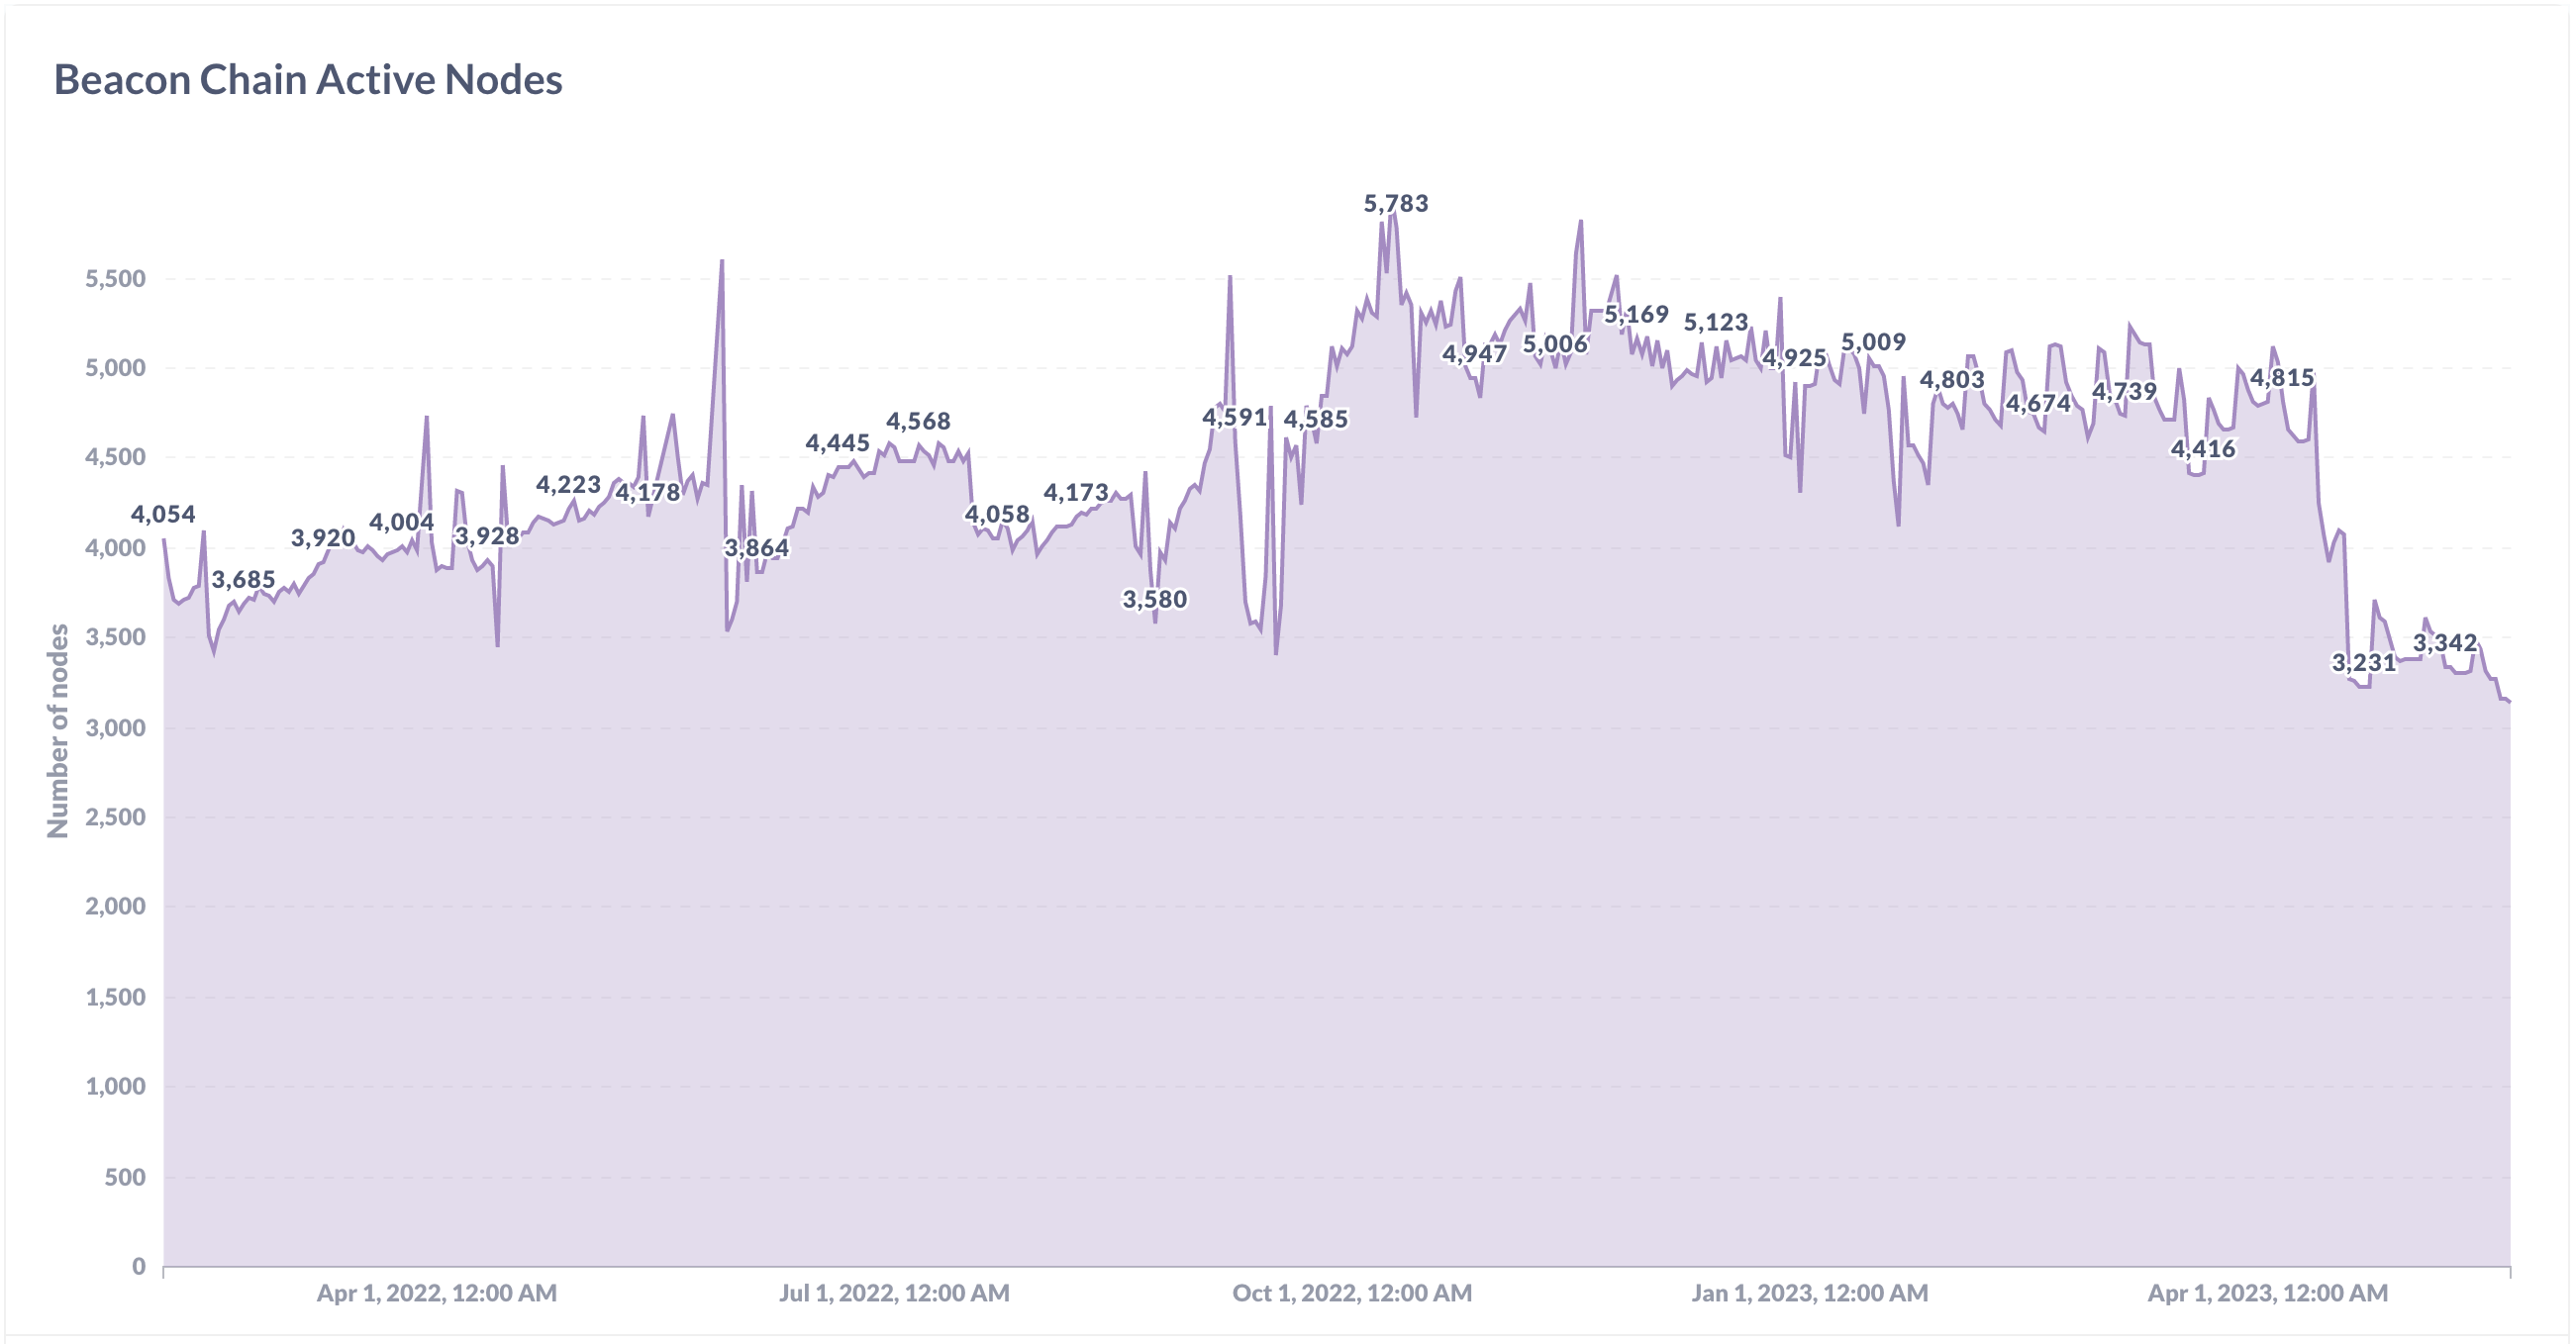
\includegraphics[width=0.48\linewidth]{images/activenodes}
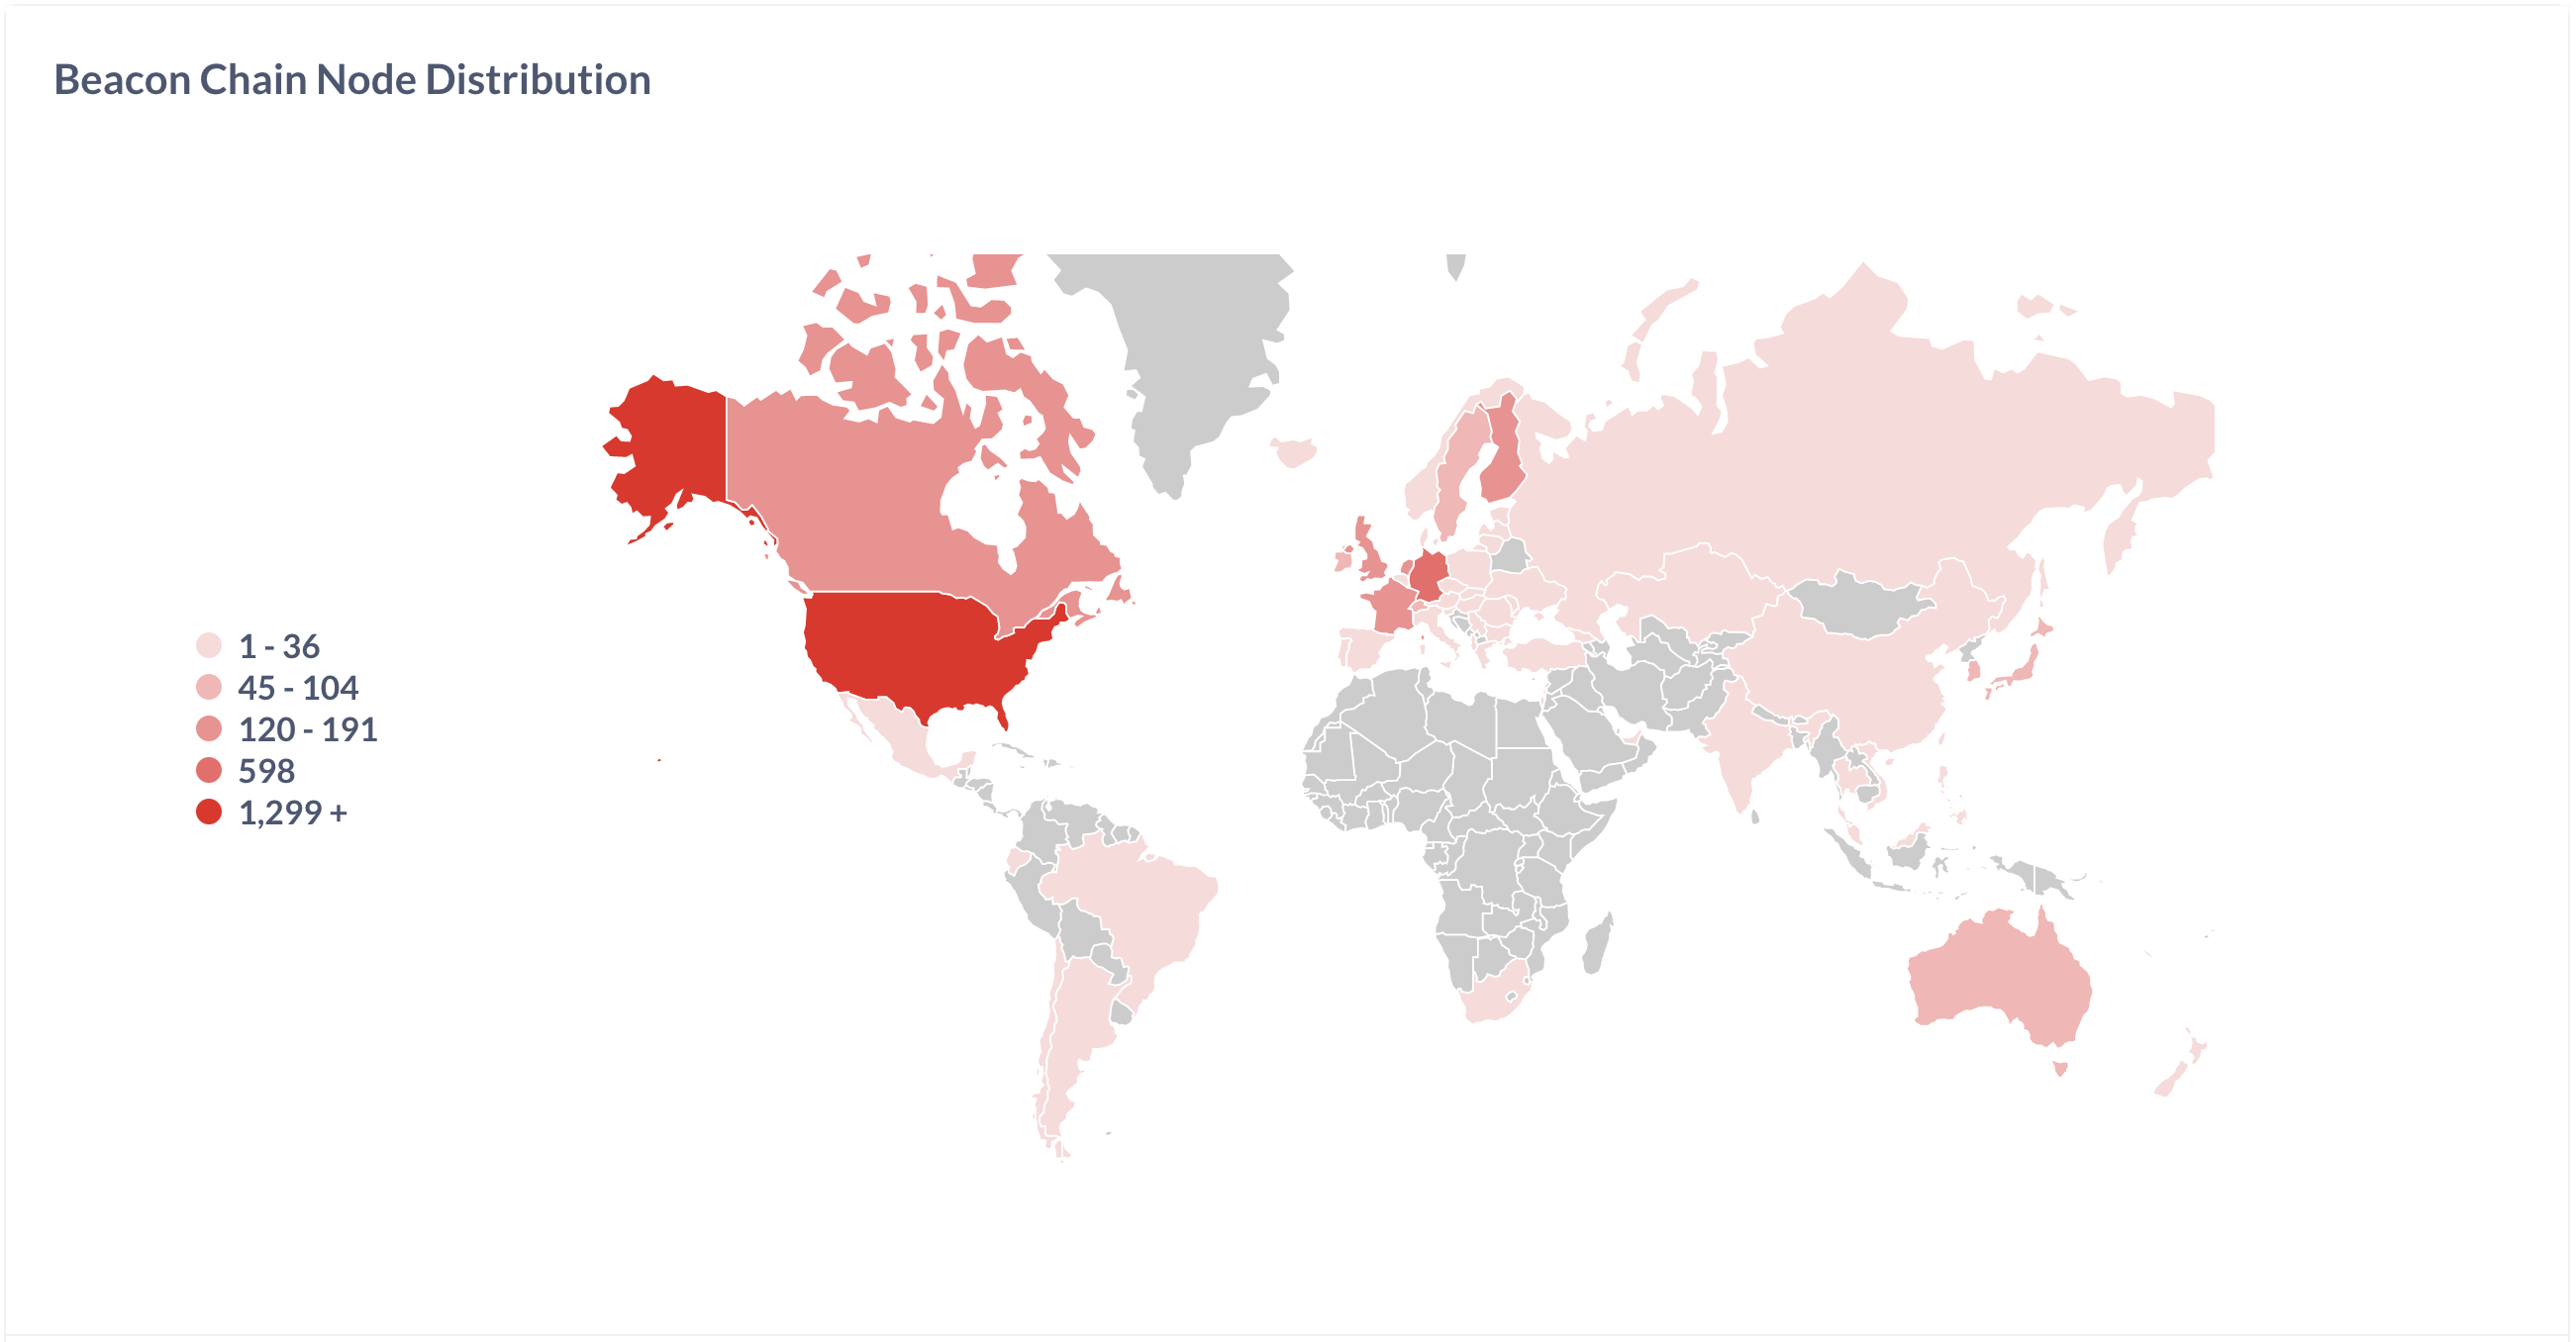
\includegraphics[width=0.48\linewidth]{images/evolution} \\
(a)\hspace{160pt}        (b)\\
\caption{Operating system distribution of active beacon chain nodes from Migalabs (a) and client diversity evolution of beacon chain nodes (b) (9 May 2023)}
\label{fig:active}
\end{center}
\end{figure}

\begin{figure}[htbp]
\begin{center}
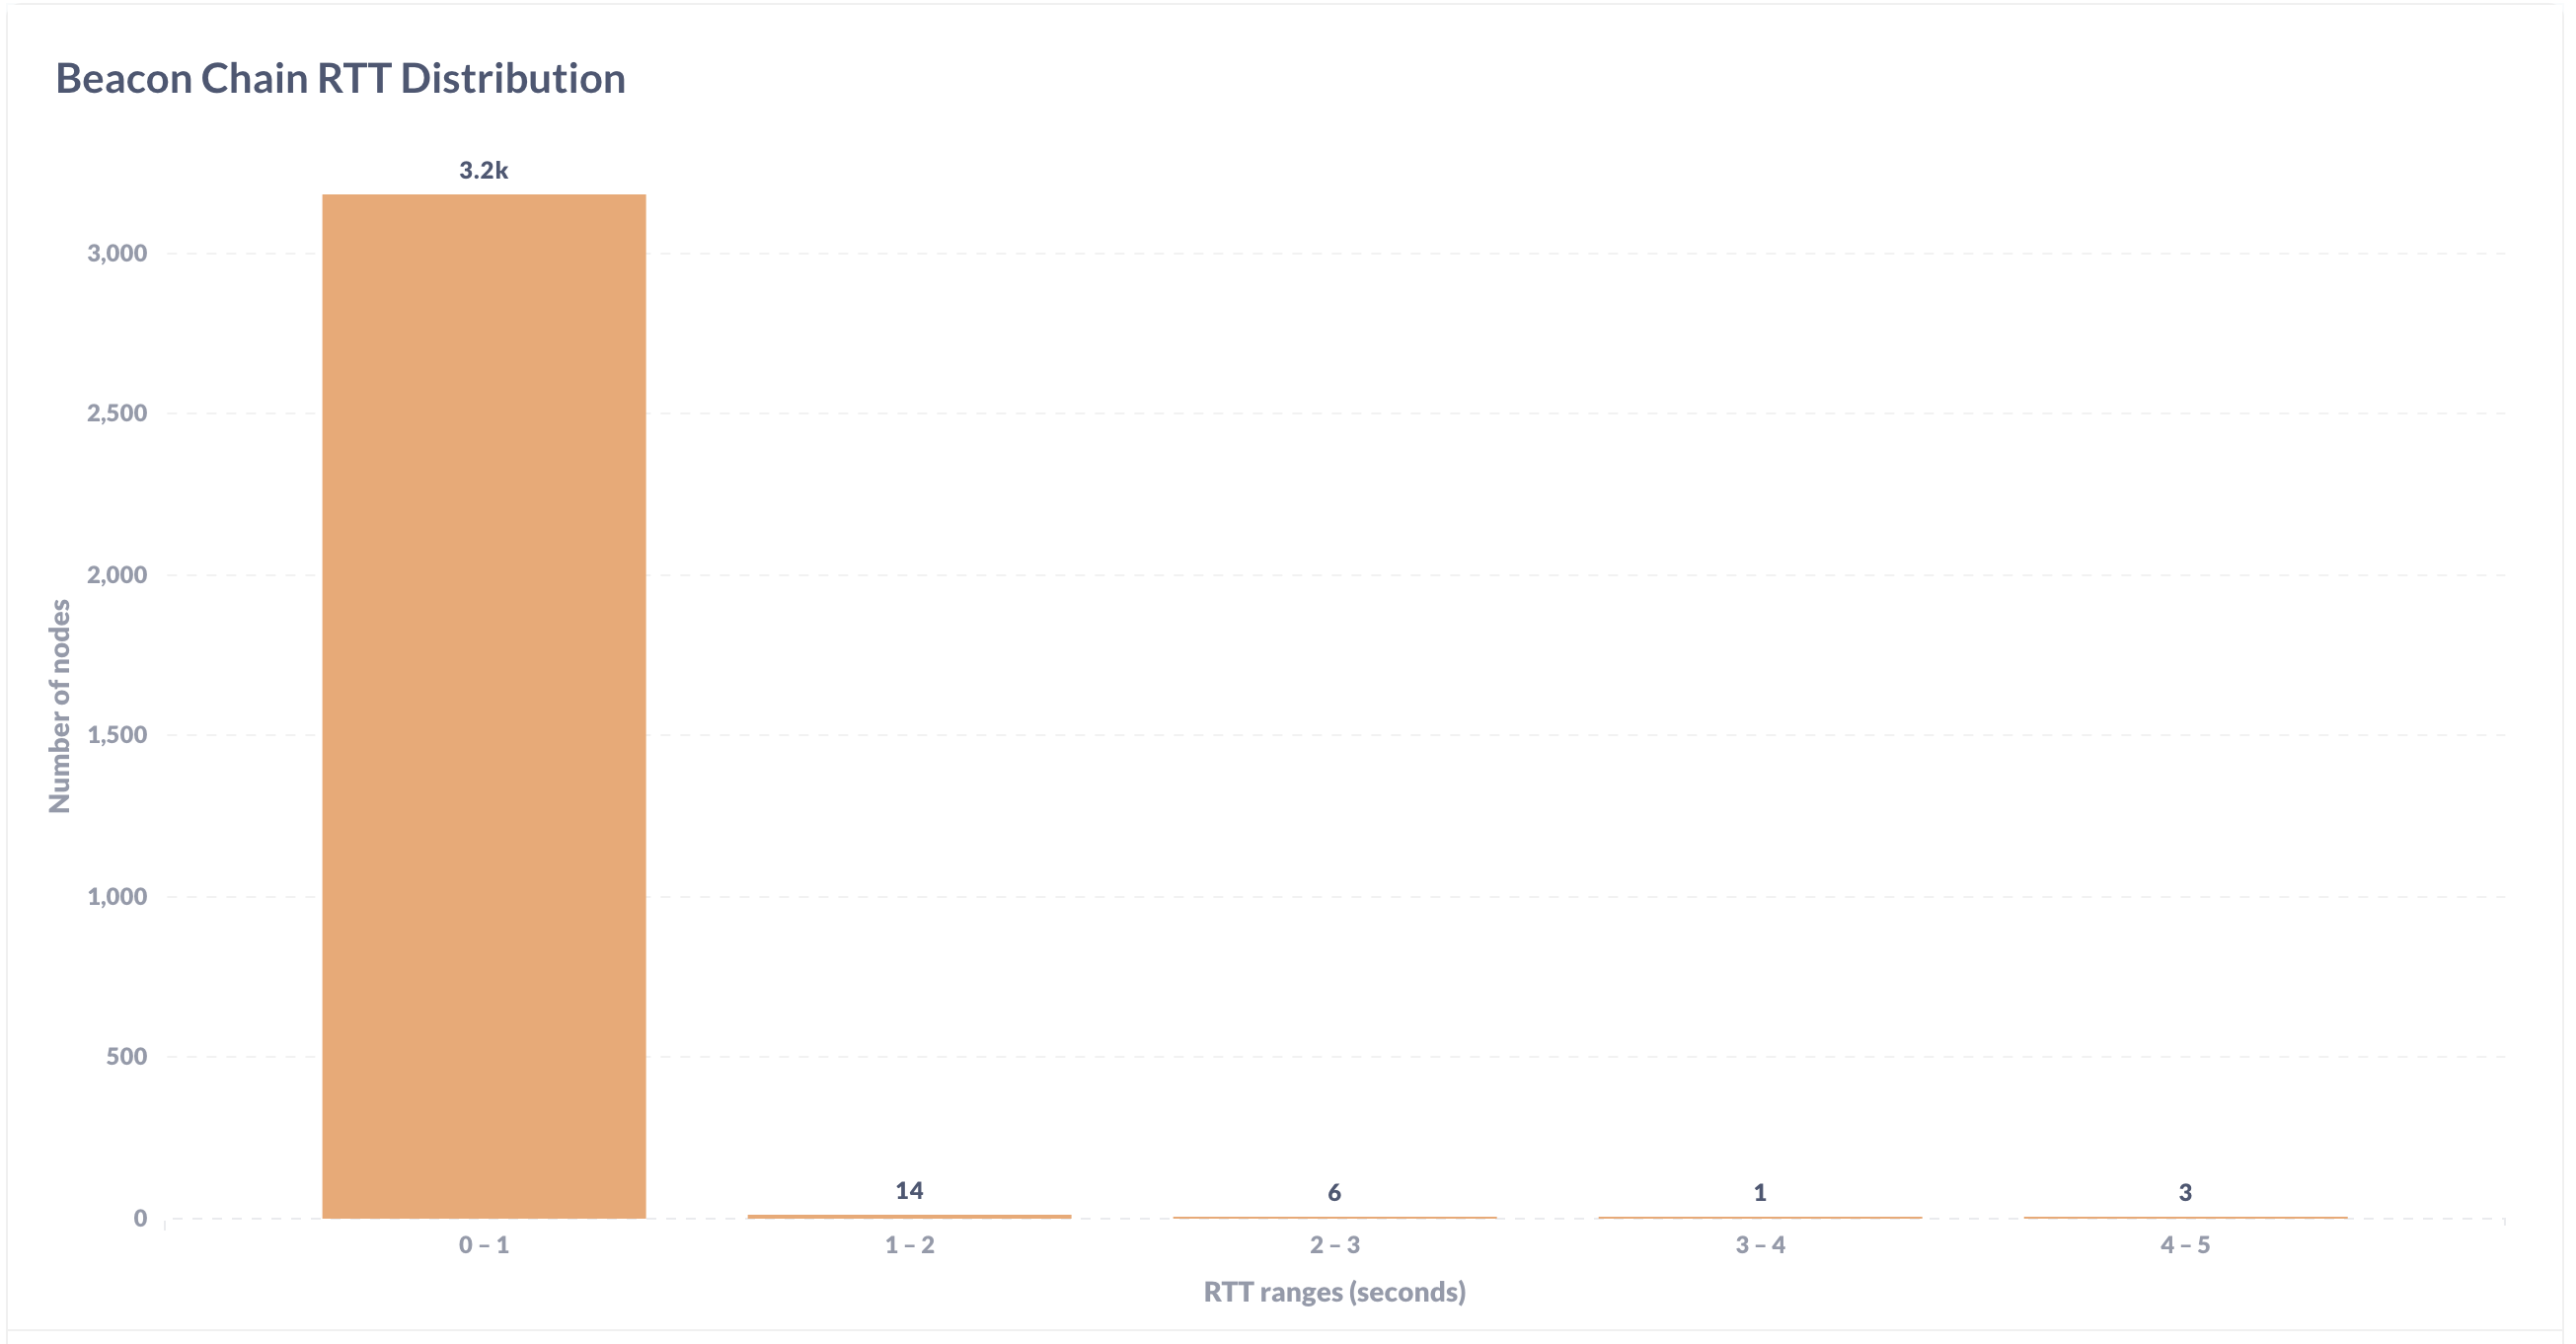
\includegraphics[width=0.48\linewidth]{images/activertt}
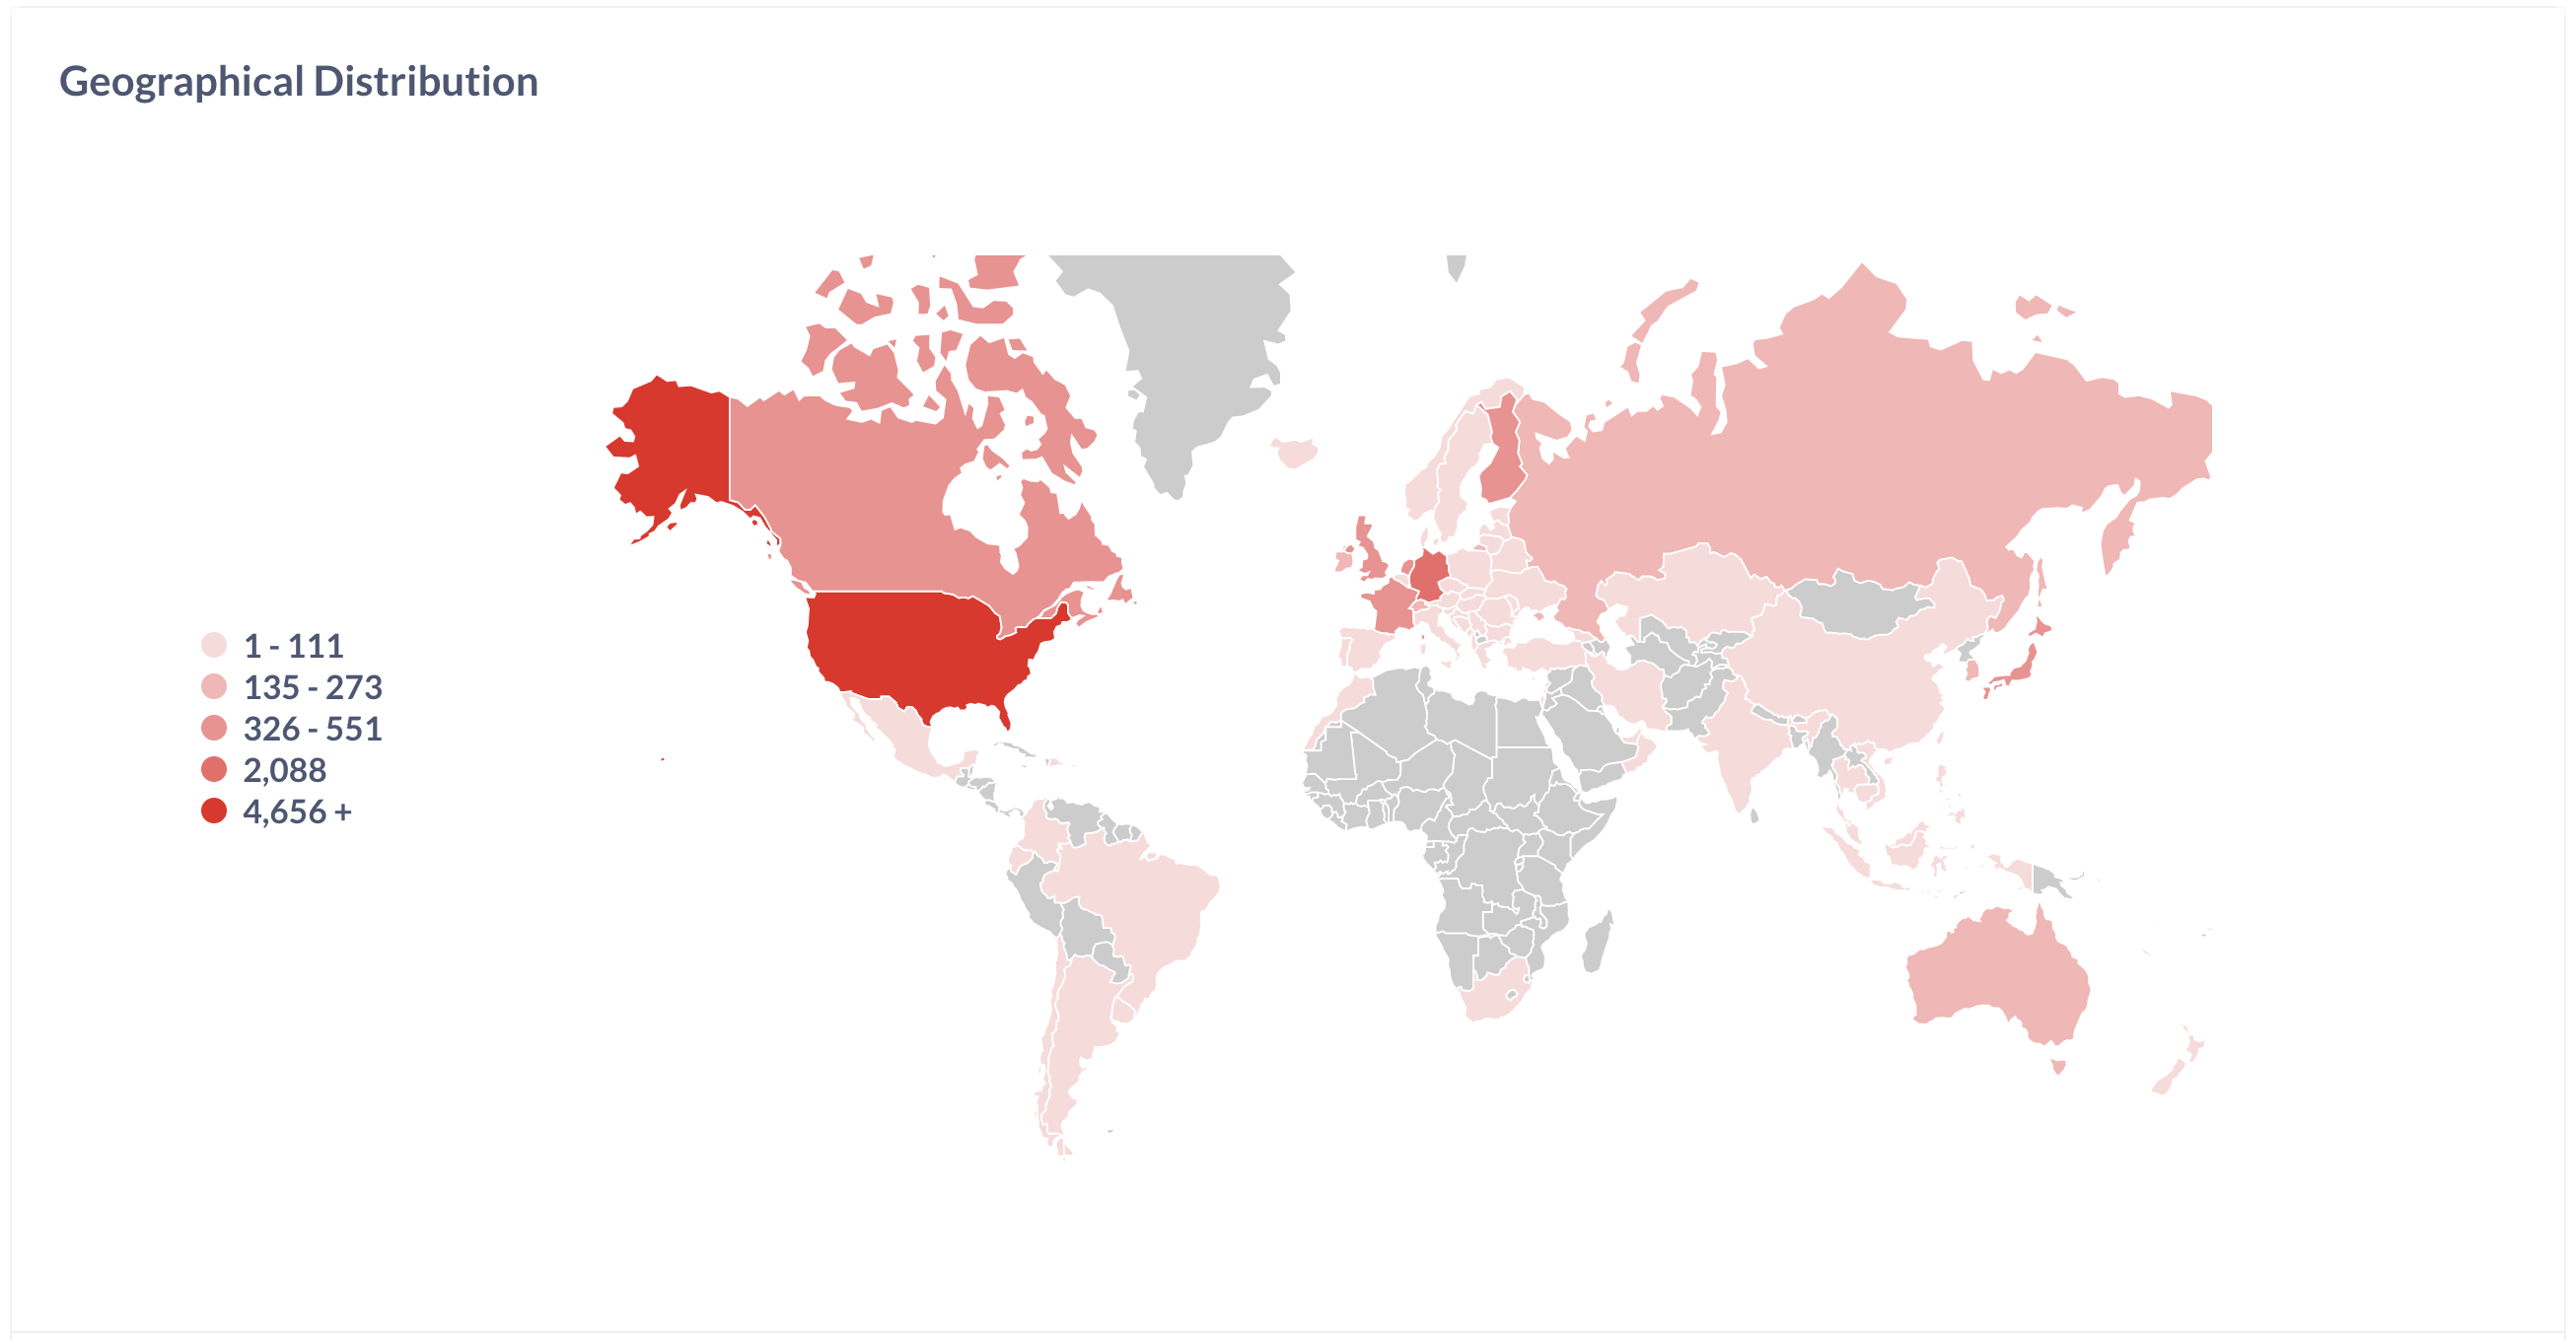
\includegraphics[width=0.48\linewidth]{images/geographical} \\
(a)\hspace{160pt}        (b)\\
\caption{Distribution of active beacon chain nodes round trip time (RTT) from Migalabs (a) and geographical distribution (b) (9 May 2023)}
\label{fig:rtt}
\end{center}
\end{figure}

\begin{figure}[htbp]
\begin{center}
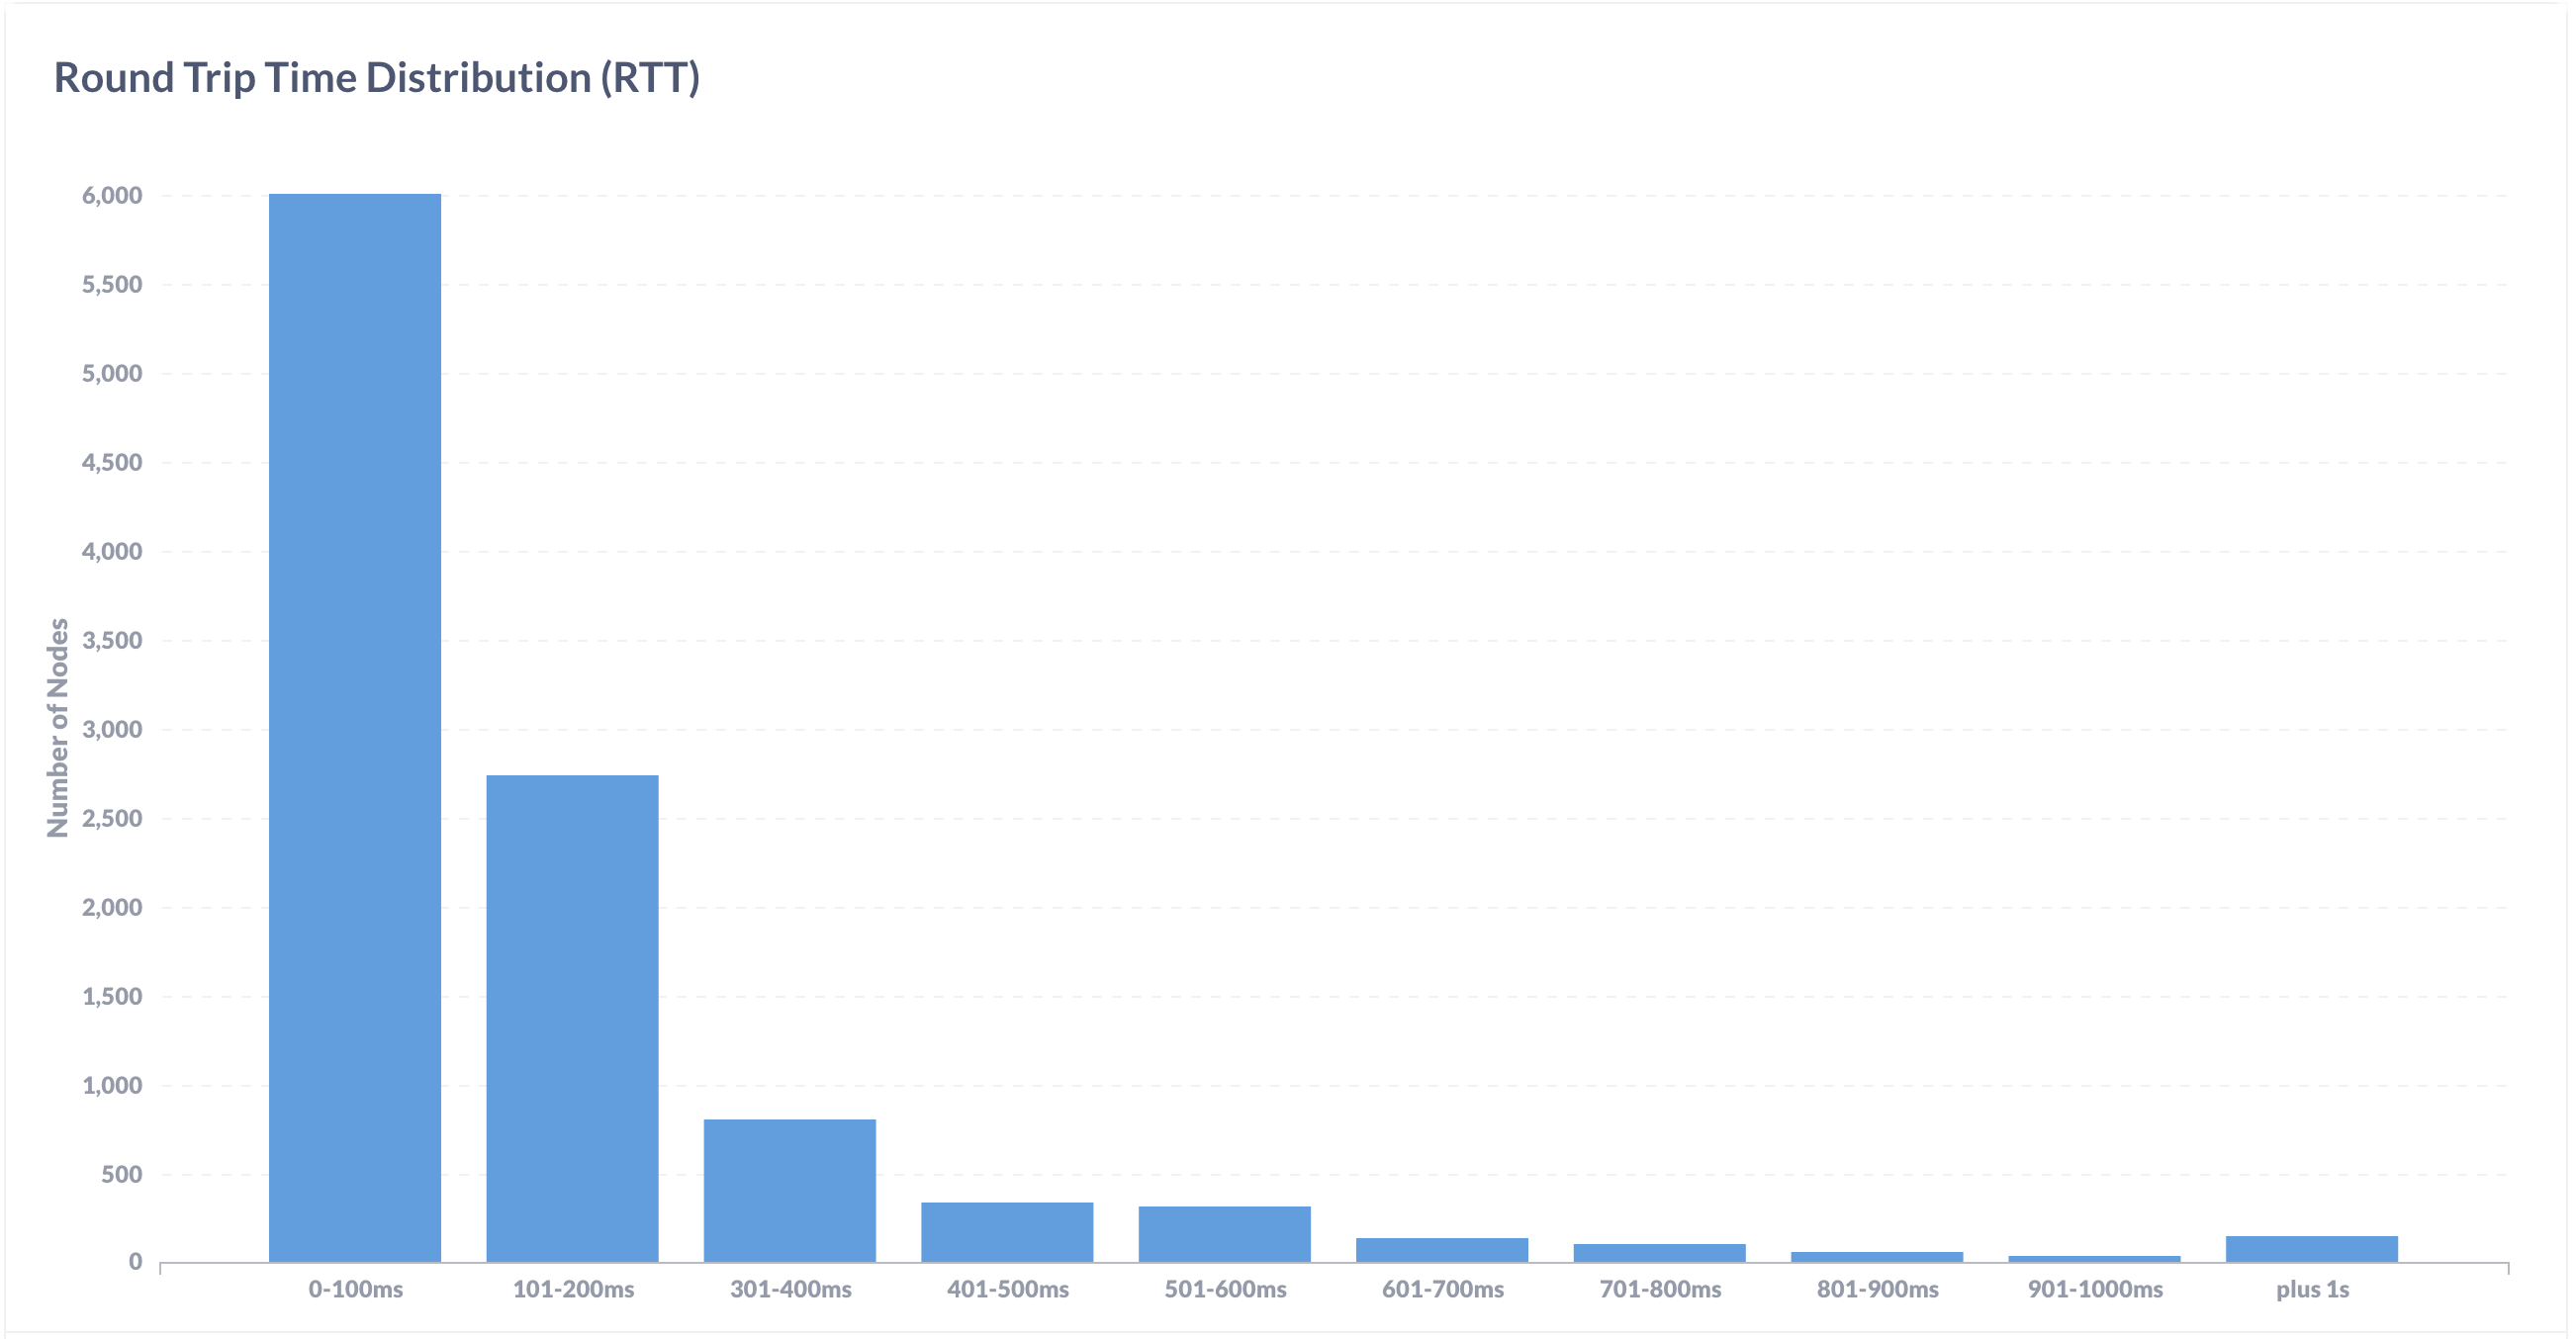
\includegraphics[width=0.48\linewidth]{images/rttdist}
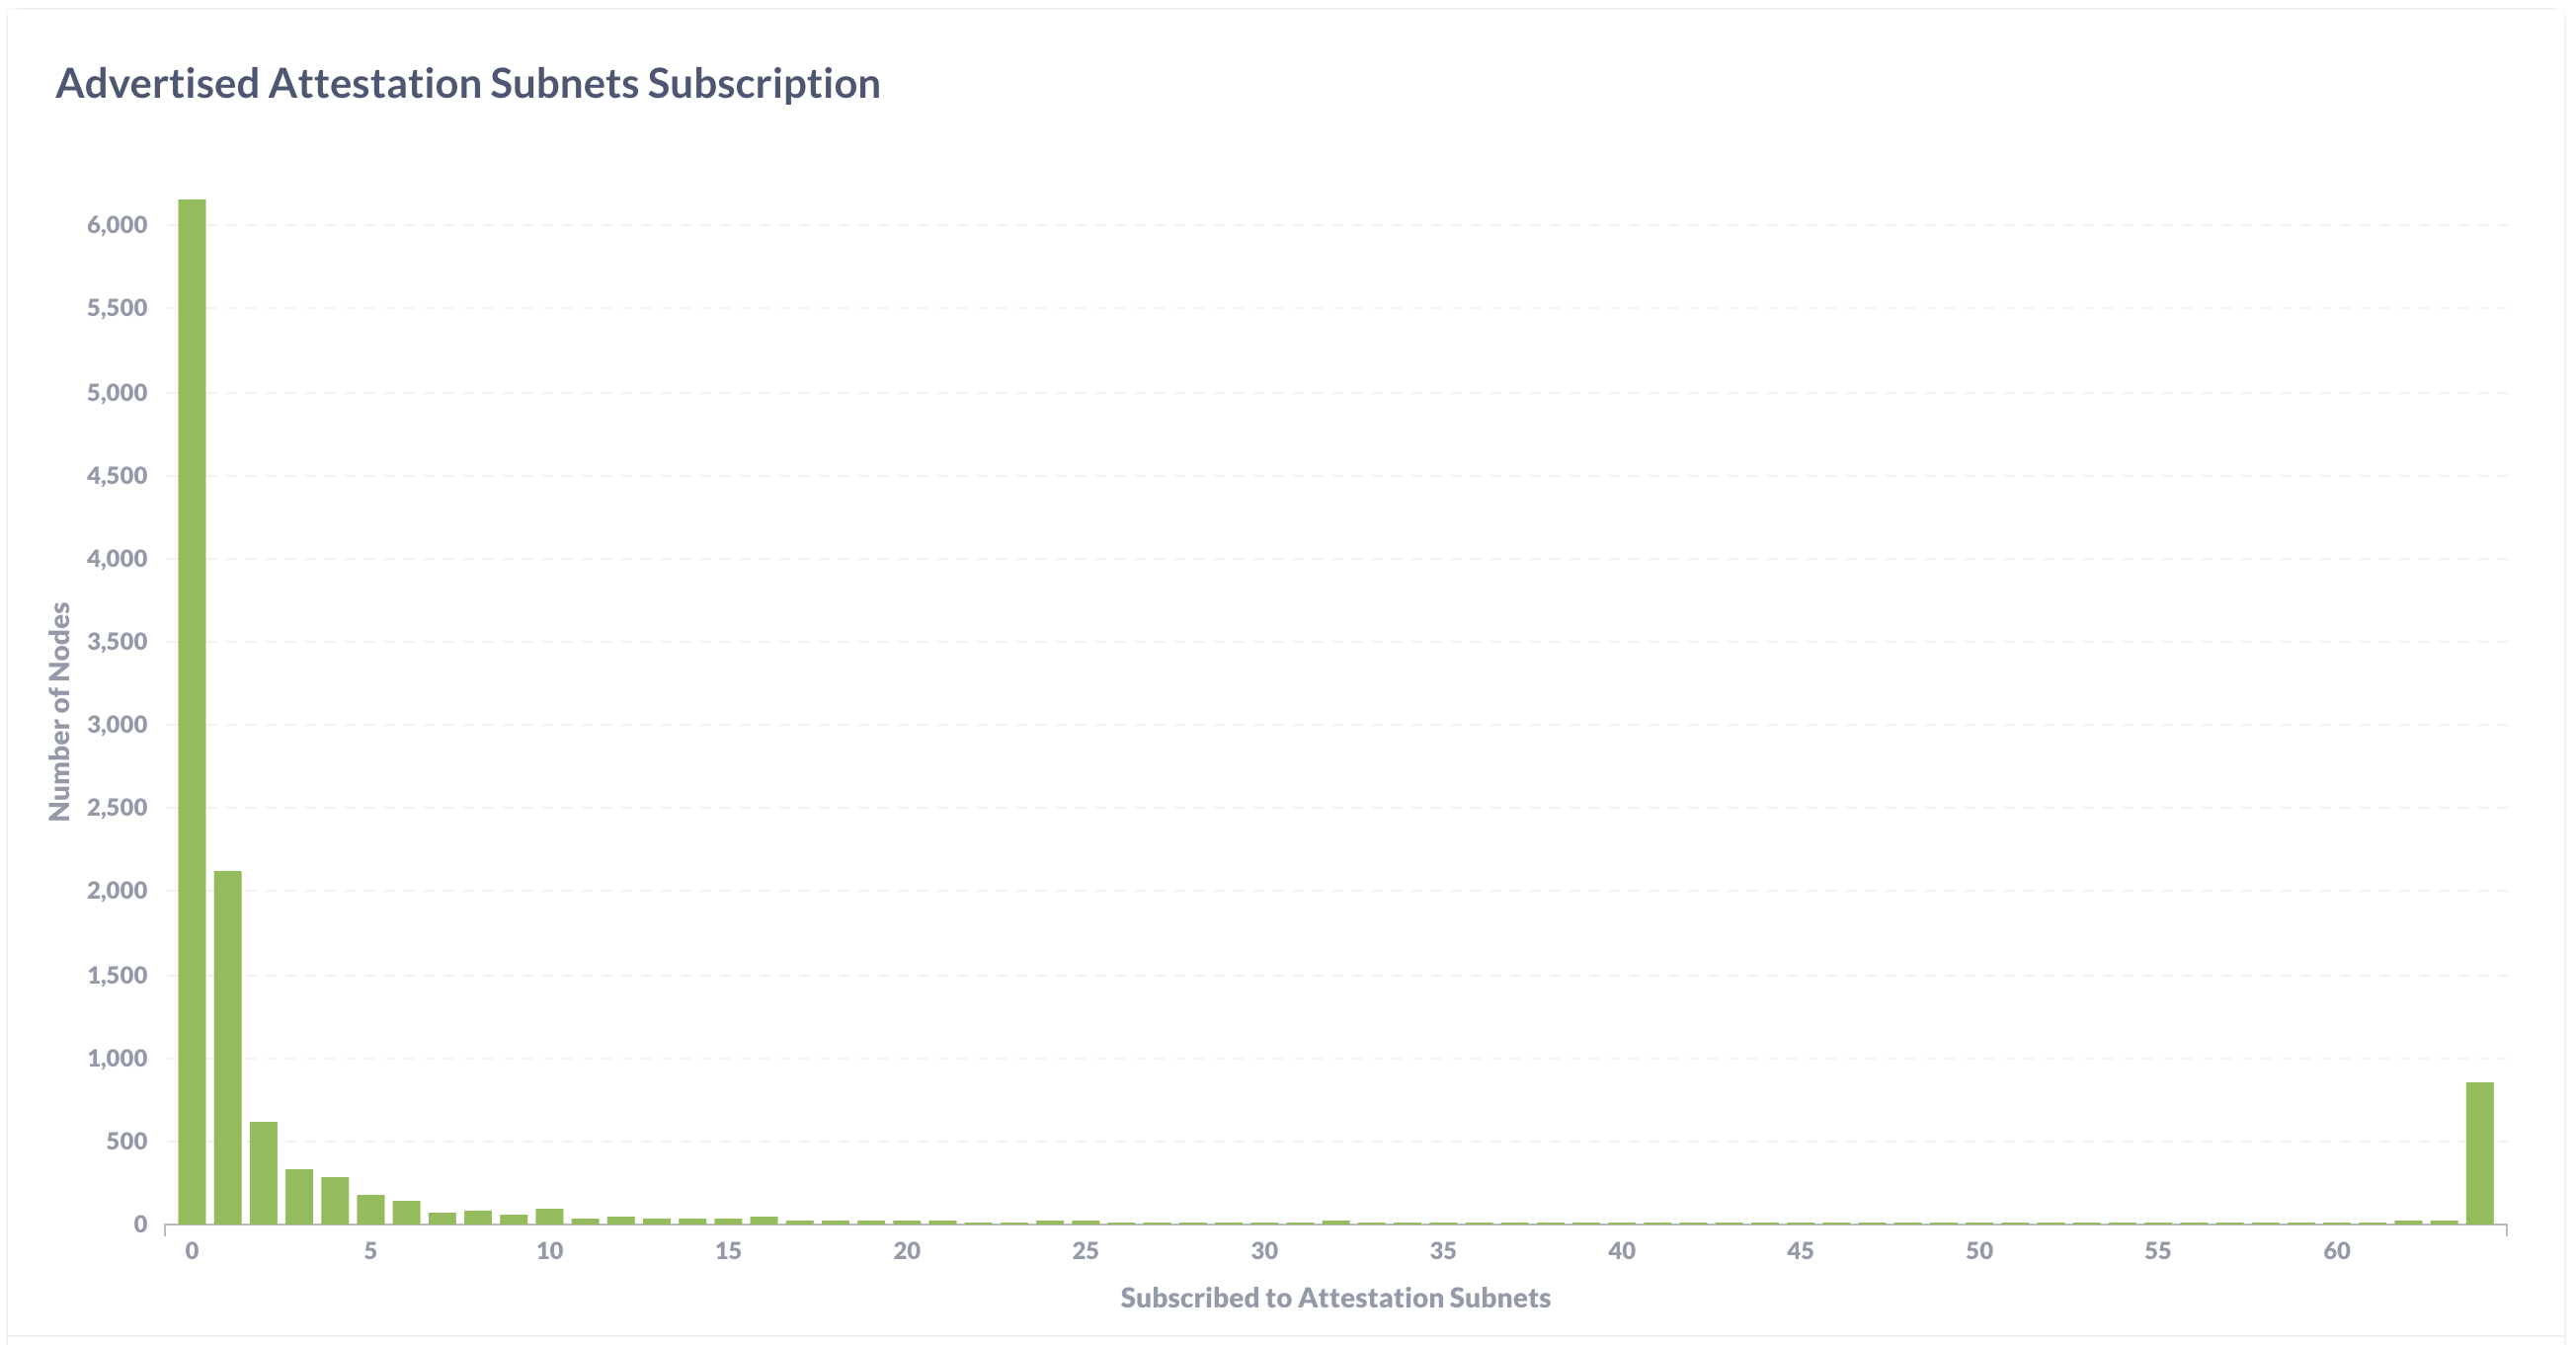
\includegraphics[width=0.48\linewidth]{images/aass} \\
(a)\hspace{160pt}        (b)\\
\caption{Distribution of active beacon chain nodes round trip time distribution (RTT) from Migalabs (a) and advertised attestation subnets subscription (b) (9 May 2023)}
\label{fig:aass}
\end{center}
\end{figure}

\begin{figure}[htbp]
\begin{center}
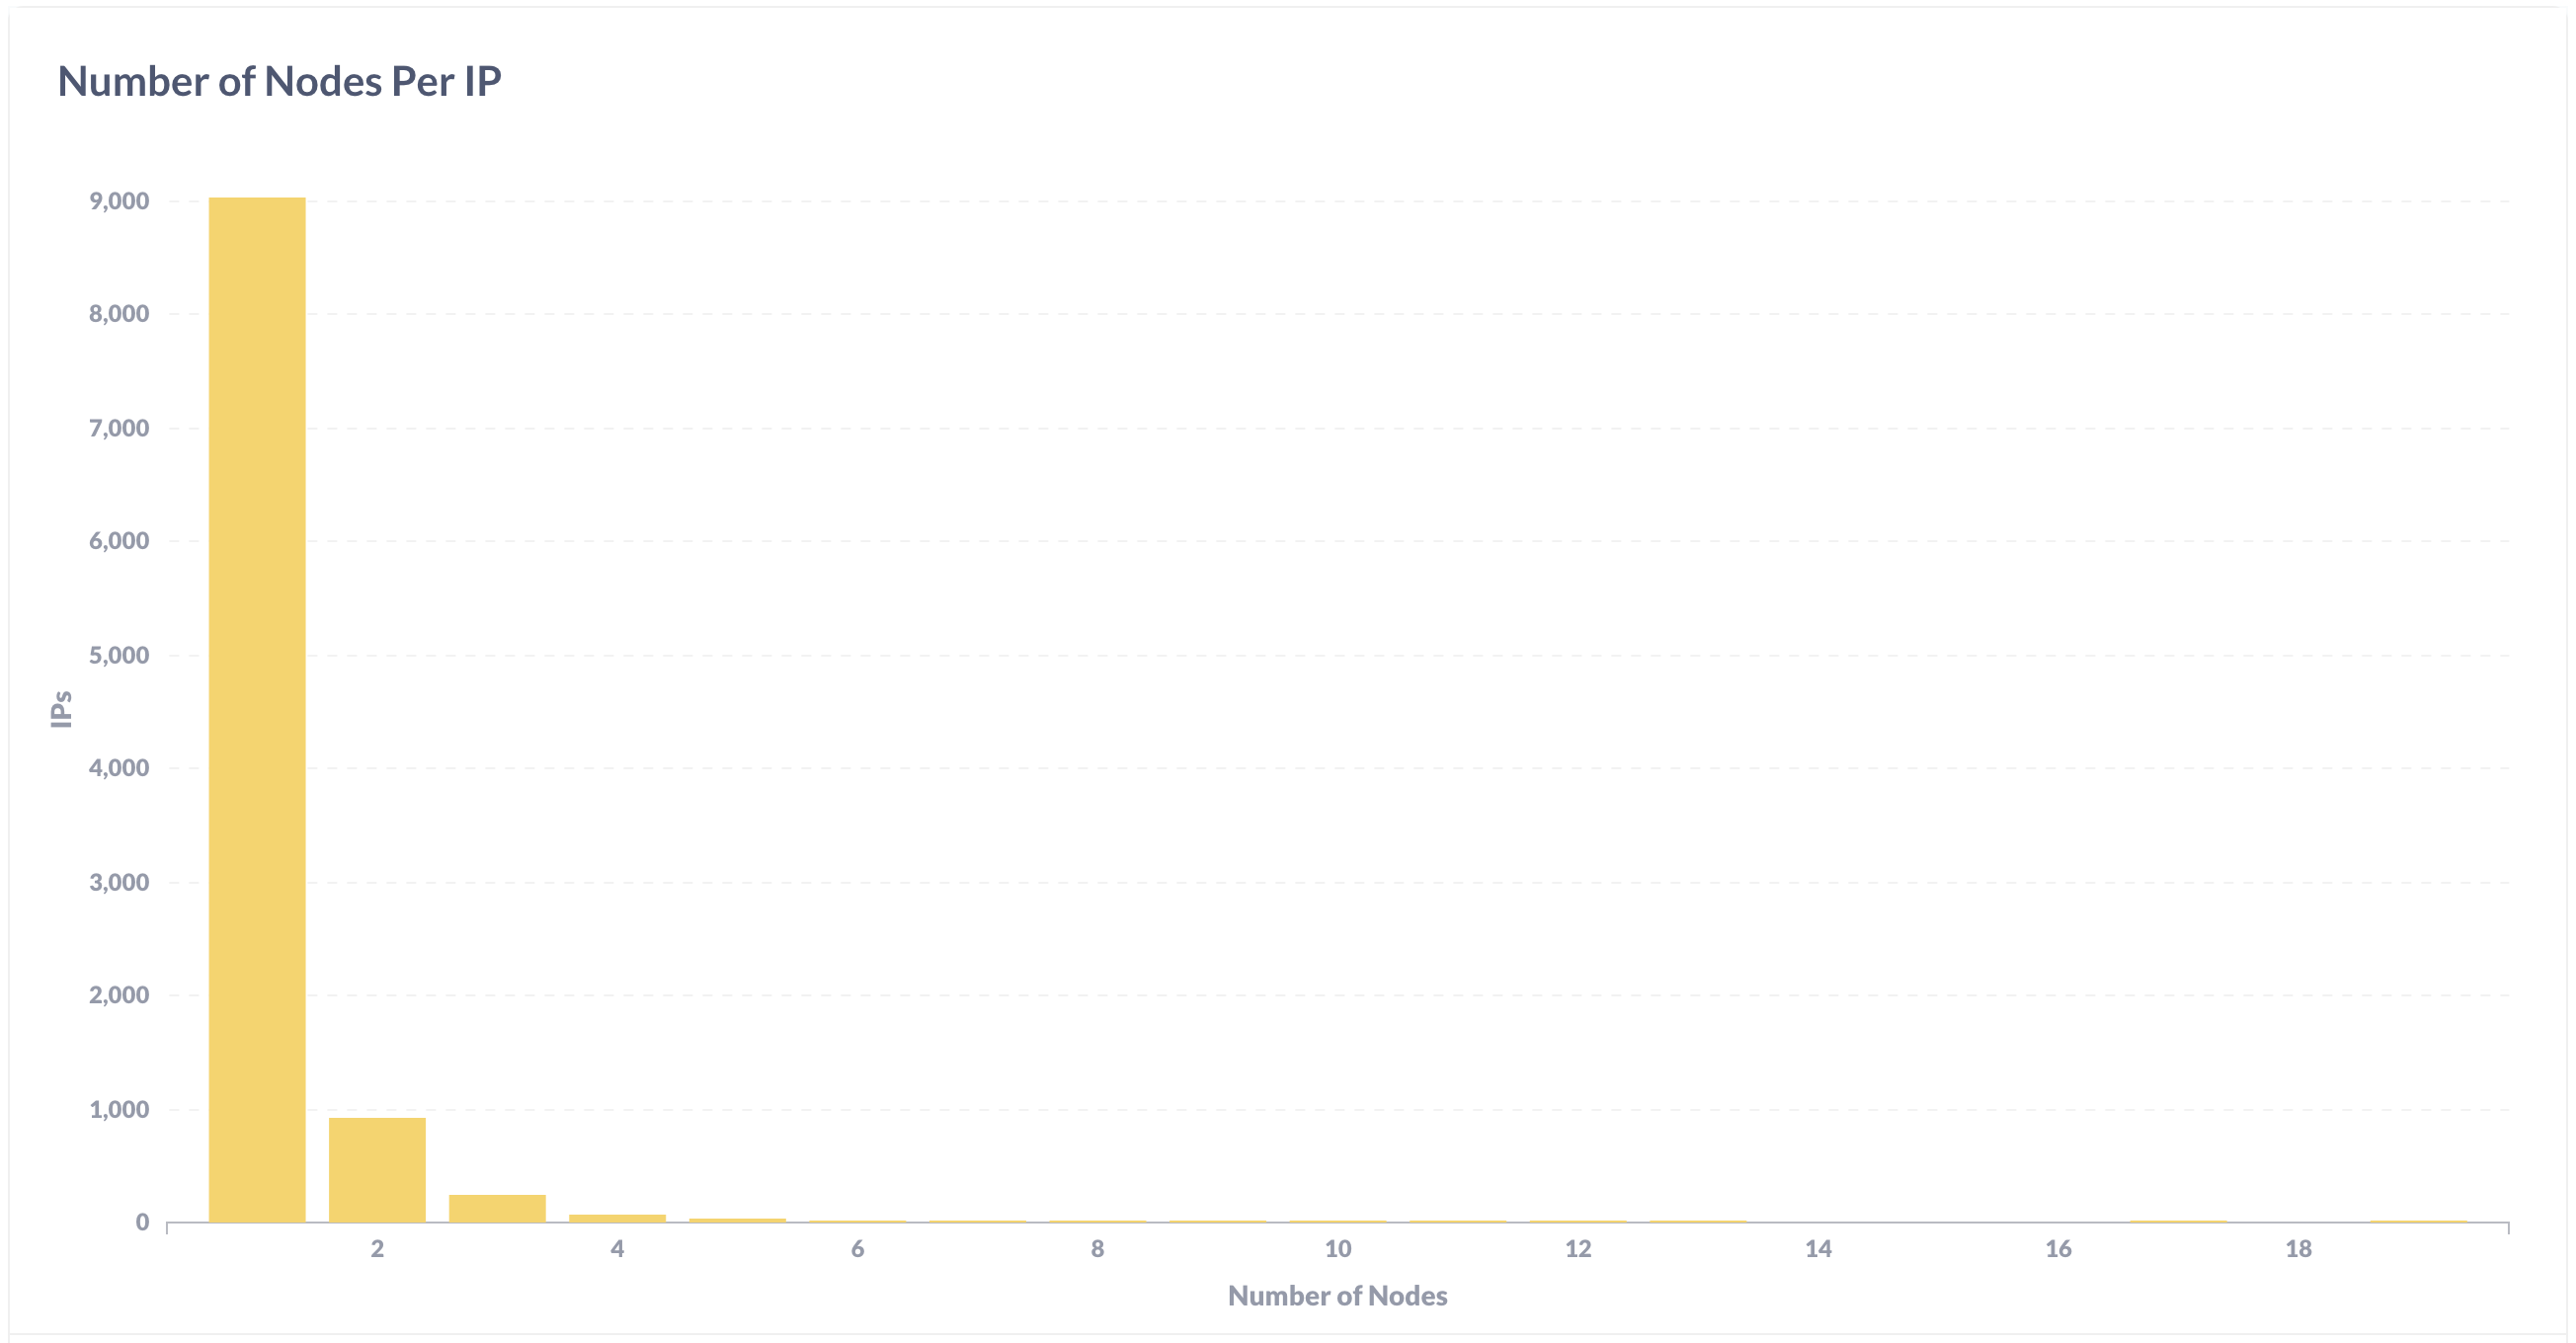
\includegraphics[width=0.48\linewidth]{images/ipdist}
\caption{Number of beacon nodes per IP from Migalabs }
\label{fig:ipdist}
\end{center}
\end{figure}


\end{document}
